% This is LLNCS.DEM the demonstration file of
% the LaTeX macro package from Springer-Verlag
% for Lecture Notes in Computer Science,
% version 2.4 for LaTeX2e as of 16. April 2010
%
\documentclass{llncs}
%
\usepackage{makeidx}  % allows for indexgeneration
%

\usepackage{amsmath}
\usepackage{graphicx}
\usepackage{pgfplots}
\usepackage{tikz}
\bibliographystyle{apalike}
\usetikzlibrary{shapes,arrows}
\usetikzlibrary{calc,patterns,snakes,decorations.pathmorphing,decorations.markings}
\usetikzlibrary{positioning}

\begin{document}
%
%\frontmatter          % for the preliminaries
%
%\pagestyle{headings}  % switches on printing of running heads
%\addtocmark{Hamiltonian Mechanics} % additional mark in the TOC
%
\vspace{1cm}
%\begin{flushright}\noindent
%April 1995\hfill Walter Olthoff\\
%Program Chair\\
%ECOOP'95
%\end{flushright}
%


\begin{abstract}
\end{abstract}
\section{Introduction}

In this work , we will try to design fuzzy based controllers to drive race cars in TORCS simulator:\\
AD1: Speed  based fuzzy controller using the track sensors.
AD2: Speed and steer based fuzzy controller using the track sensors.\\
AD3: Speed and steer based fuzzy controller using the turning radius.\\
AD5: Speed and steer based fuzzy controller using the track sensors and consideration of opponents position in the track.

\section{The Open Racing Car Simulator "TORCS"}
\subsection{TORCS Presentation}

The Open Racing Car Simulator) is a free three-dimensional racing video game.
Even if it has not the graphic quality of commercial games, TORCS allows to play different races, about forty vehicles , on a wide variety of tracks (dusty roads, highways, formula 1 circuits, etc).[\cite{manuel}]. The TORCS project was created by \textit{Eric Espié} and \textit{Christophe Guionneau} and currently \textit{Bernhard Wymann}, \textit{Christos Dimitrakakis}  and other contributors continue to develop it. [\cite{manual}]



TORCS1 (The Open Racing Car Simulator) is one of the most popular car racing simulators. It is written in C++ and
is available under GPL license front its web page. TORCS
presents several advantages for academic purposes, such as:
\begin{enumerate}
	
	\item  It lies between an advanced simulator, like recent commercial
	car racing games, and a fully customizable environment,
	like the ones typically used by computational
	intelligence researchers for benchmark purposes.
	\item  It features a sophisticated physics engine (aerodynamics,
	fuel consumption, traction,...) as well as a 3D graphics
	engine for the visualization of the races.
	\item  It was not conceived as a free alternative to commercial
	racing games, but it was specifically devised to make it
	as easy as possible to develop your own controller In fact, controllers are implemented as separated software
	modules ,so it is easy to develop a new controller and to plug
	it into the game.
	
\end{enumerate}

TORCS has several different cars with real characteristics(fuel consumption, aerodynamics, collisions or traction) (see Fig.\ref{car}) and different tracks [\cite{manuel} ]( See fig. \ref{trackexp} and Table\ref{CATRA}). The user can create his own track with the track editor.

\begin{figure}[h!]
	\centering
	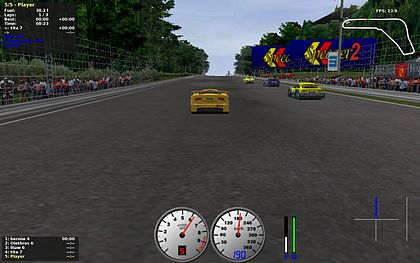
\includegraphics[width=0.5\textwidth]{fig/TORCS1.PNG}
	\begin{minipage}{10cm}
		\centering
		
		\caption{\footnotesize TORCS race}
		\label{0301}
	\end{minipage} 
\end{figure}

\begin{figure}[h!]
	\centering
	\label{voiture}
	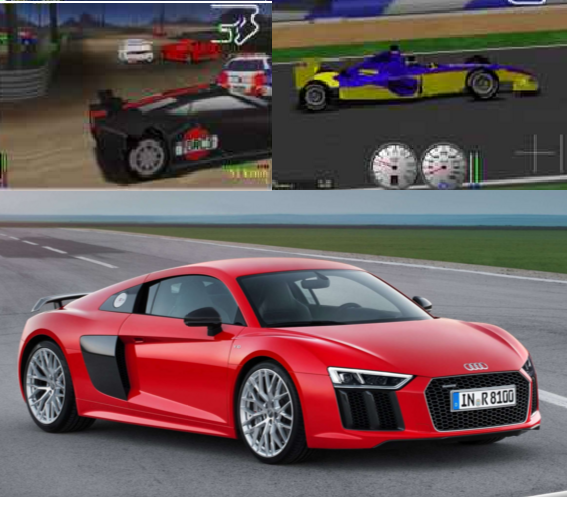
\includegraphics[width=0.4
	\textwidth]{fig/voiture.PNG}
	\includegraphics[width=0.45\textwidth]{fig/NASCAR.PNG}
	\begin{minipage}{10cm}
		\centering
		
		\caption{\footnotesize TORCS race car}
		
	\end{minipage} 
\end{figure}

\begin{table}[h!]
	
	\caption{TORCS Tracks }
	\label{CATRA}			
	%Tracks                  	
	\begin{tabular}{ |p{1cm}|p{3cm}|p{3 cm}|p{2 cm}|p{2 cm}|}
		{ \textbf{Num} }&	
		{ \textbf{Name} }&
		{ \textbf{Author}}&  
		{ \textbf{Length(m)} } &
		{ \textbf{Width (m)} }
		\\
		\hline
		1 & CG Speedway nember1 & B.Wymana & 2057 & 15 
		\\
		\hline
		2 & CG Track 2/1 & CG & 3185/2843 & 15/10 
		\\
		\hline
		3 & Olethos Road1 & C.Dimitrakakis & 6282 & 10 
		\\
		\hline
		4 & RuudsKongen & A.Summer & 3274 & 11
		\\
		\hline
		5 & Spring & E.Espie & 22129 & 12
		\\
		\hline
		6 & Steer1 & A.Summer & 38423 & 14
		\\
		\hline
		7 & Whell1 & E.Espie B.wymann & 4328 & 14
		\\
		\hline	
		8 & Whell2 & A.Summer & 6205 & 12
		\\
		\hline	
		9 & Alborg & E.Espie B.wymann & 2587 & 10
		\\
		\hline
		10 & Apline 1 & E.Espie  & 6355 & 12
		\\
		\hline
		11 & Apline 2 & D.schellhammer & 3773 & 10
		\\
		\hline
		12 & Brondehach & E.Summer & 3919 & 13
		\\
		\hline
		13 & Crokscrew & Kilo,andrew & 3608 & 12
		\\
		\hline
		14 & Etrack [1-6] & E.Espie B.wymann& [3000-7000] & 12/13
		\\
		\hline
		15 & ERoad  & E.Espie B.wymann & 3270 & 16
		\\
		\hline	
		16 & Forza  & A.Summer & 5784 & 11
		\\
		\hline   		    	
	\end{tabular} 
	
\end{table}

\begin{figure}[ h!]
	\centering
	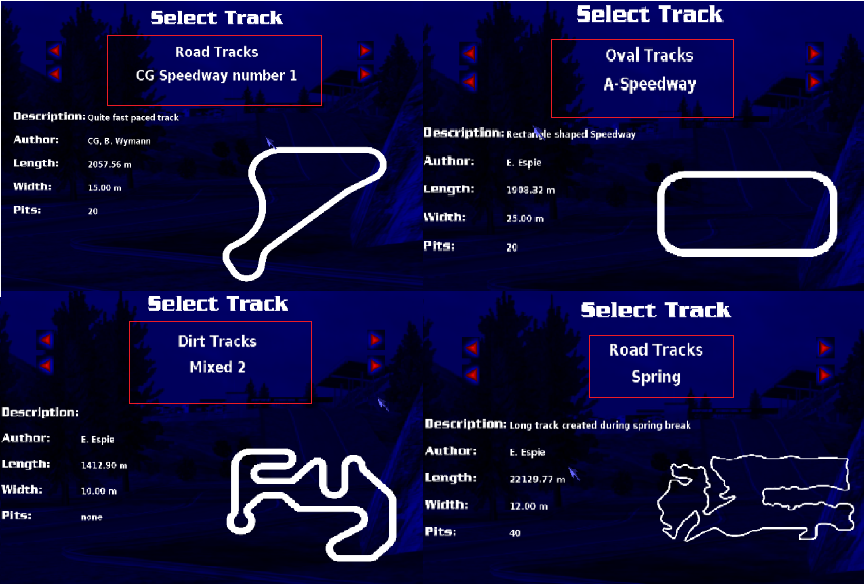
\includegraphics[width=0.6\textwidth]{fig/trackexp.PNG}
	\begin{minipage}{10cm}
		\centering
		\caption{\footnotesize TORCS's tracks}
		\label{trackexp}
	\end{minipage} 
 
	
\end{figure}
\newpage

The drivers in TORCS can practice and test their controllers and can participate in three main kinds of races:
\begin{itemize}
	\item \emph{Warm-up}: 
	The driver is able to explore the track and extract the information it contains for a limited time; 
	\item \emph{Qualifiers}: 
	Time trial race where drivers try to get the fastest time.
	\item \emph{Real race}: 
	
	The best eight drivers in the qualifiers can participate in a a final race to get the winner.			
\end{itemize}

\subsubsection{TORCS controller definition}	
A robot is a program run from TORCS that drives a car. It gets as input information about the current state of the car and its situation on the track. These collected data are used to compute actions to do in the next simulation tick; like steer, gear changes, acceleration or brake and clunch. A client may request a restart of the race by sending a special action on the server: Resatart or shutdown.
[\cite{manual}]
\subsection {TROCS Architecture}
The Open Racing Car Simulator (TORCS) is a standalone application where robots are built as separate modules loaded into the main memory when a race takes place. [\cite{Torcs3} ]
This simulator includes the original architecture of TORCS in three ways: [\cite {manual}]
\begin{enumerate}
	\item TORCS is a client-server applications, robots (bots) are run in external processes connected to the server running across by the UDP connections.\\
	
	\item The simulation is achieved in real time and  game ticks are approximately 20 ms of simulated time, the server sends the current sensors values to each robot and waits 10 ms (real time) to receive an action from the bot.
	If no action is happened, the simulation continues and the last action will be used.\\
	
	\item The "TORCS" software make a physical separation between the driver code and running server, it builds an abstract layer that gives complete freedom of choice of programming language that will be used for robots and limit access only to information defined by the designer (the data encapsulation) See Figure ~\ref{architorcs}.
\end{enumerate}
\begin{figure}[h!]
	\centering
	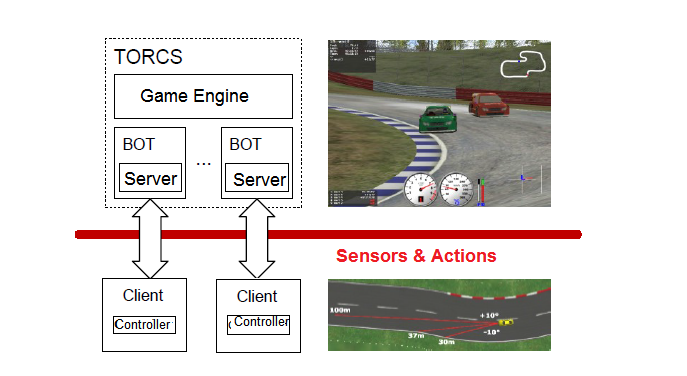
\includegraphics[width=1.1\textwidth]{fig/arch2.PNG}
	\begin{minipage}{10cm}
		\centering
		
		\caption{\footnotesize TORCS Architecture}
		\label{architorcs}
	\end{minipage} 
\end{figure}

\subsection{Sensors and Actuators}
The TORCS software creates a physical separation between the game engine and pilotes.Ainsi to develop a robot it is not necessary to have any knowledge a
about the engine TORCS or internal data structure.[\cite{torcs2012}]\\

In the competition, The robot perceives the racing environment through a number of sensors that provide information about the state of the car (the current speed, fuel level, ...), the state of the race (current lap, the elapsed distance,...), opponents positions and track borders, ... these data enable the designer to form a base of solutions to achieve a typical driving. [\cite{manuel}] [\cite{torcs2}]		\\		
Tables ~\ref{t1} present a complete list of available sensors with a description of each one.[\cite{Torcs3}]\\

\begin{table}[h!]
	
	\begin{tabular}{|p{2cm}|p{3cm}|p{3 cm}|p{4 cm}|}
		\hline
		{\textbf{Sensor} }&
		{\textbf{Name} }&
		{\textbf{Range} (unit)} &  
		{\textbf{Data type}}\\ 
		\hline
		1 & Angle & [-$\pi$,+$\pi$ ] & Double\\ 
		\hline
		2 & curLapTime & [0,+$\infty$) (s)	& Double\\ 
		\hline 
		3 & damage & [0,+$\infty$)(point)& Double\\ 
		\hline 
		4 & distFromStart & [0,+$\infty$) (m)& Double \\ 
		\hline 
		5 & distRaced &[0,+$\infty$) (m)& Double\\
		\hline 
		
		6 & focus & [0,200] (m)& Double\\
		\hline 
		
		7 & fuel & [0,+$\infty$) (l)& Double\\
		
		\hline
		8 & gear & \{-1,0,1,.. 6\}g& Integer \\
		
		\hline
		9 & lastLapTime &[0,+1] (s) & Double \\
		
		\hline
		10 & opponents &[0,200] (m)& Double \\
		
		\hline
		10 & racePos & \{1,2,...,N\} & Double \\
		\hline
		11 & rpm    & [0,+$\infty$) (rpm)   & Double \\
		\hline  
		13 & speedX & (-$\infty$,+$\infty$) (km/h) & Double\\
		\hline  
		14 & speedY &(-$\infty$,+$\infty$) (km/h)  & Double\\
		\hline 
		15 & speedZ & (-$\infty$,+$\infty$) (km/h) & Double \\
		
		\hline
		16 & track &  [0,200 ] & Double\\ 
		\hline
		17 & trackPos & (-$\infty$,+$\infty$) & Double\\
		
		\hline
		
		18 & wheelSpinVel  & [0,+$\infty$) (rad/s) & Double\\
		
		\hline
		19 & z &  (-$\infty$,+$\infty$) (m) & Double\\
		
		\hline
		
	\end{tabular}
	\caption{Available TORCS sensors Description}
	\label{t1}
\end{table}
\newpage	

\subsubsection{Sensors Description:}
\begin{enumerate}
	\item \textbf{Angle:}Angle between the car direction and the direction of the
	track axis. see(fig~\ref{tab1} and fig~\ref{tab11} )
	\begin{figure}[h!]
		
		\centering
		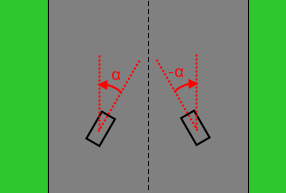
\includegraphics[width=0.7\textwidth]{fig/angle1.PNG}
		\begin{minipage}{10cm}
			\centering
			\caption{\footnotesize Angle between Car and track axis.}
			\label{tab11}
		\end{minipage} 

		
	\end{figure}
	
	\item \textbf{curLapTime:}  Time elapsed during current lap.
	\item\textbf{damage:}  Current damage of the car (the higher is the value the higher
	is the damage).
	\item \textbf{distFromStart:}  Distance of the car from the start line along the track line.
	\item \textbf{distRaced:}  Distance covered by the car from the beginning of the race.
	\item \textbf{focus:}  Denote the normalized deviation and the lateral deviation of the car with the track axis.
	-focus = 0, when the car is in the middle of the track. 
	
	-focus <0 when the car is deviated to the left.
	
	-focus <-1 or focus > 1 when the car is out of the track.(See fig~\ref{tab11})
	\begin{figure}[h!]
		
		\centering
		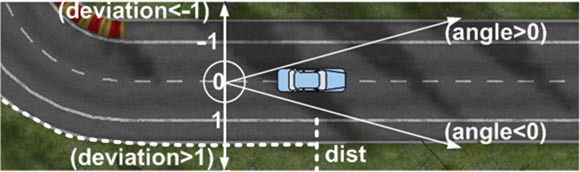
\includegraphics[width=0.8\textwidth]{fig/ANGLE.PNG}
		\begin{minipage}{10cm}
			\centering
			\caption{\footnotesize TORCS angle sensor.}
			\label{tab1}
		\end{minipage} 
		
	\end{figure}
	\item \textbf{fuel:}  Current fuel level.
	
	\item \textbf{gear:}  Current gear: -1 is reverse, 0 is neutral and the gear from 1 to 6 .
	
	\item \textbf{lastLapTime:} Time to complete the last lap
	
	\item \textbf{opponents:} Vector of 36 opponent sensors: each sensor covers a span
	of 10 degrees within a range of 200 meters and returns the
	distance of the closest opponent in the covered area. The 36 sensors cover all the space
	around the car, spanning clockwise from -180 degrees up to
	+180 degrees with respect to the car axis.(see fig.\ref{tab10})
	\begin{figure}[h!]
		\centering
		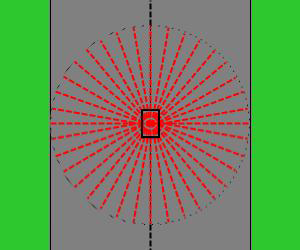
\includegraphics[width=0.4\textwidth]{fig/open.PNG}
		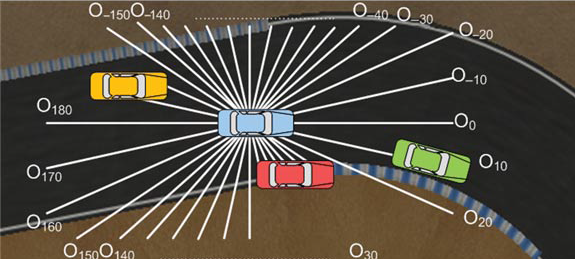
\includegraphics[width=0.4\textwidth]{fig/oppenes.PNG}
			\label{tab10}
			\caption{\footnotesize Opponents sensors.}	
	\end{figure}
	
	\item \textbf{racePos:} Position in the race with respect to other cars.(see fig.\ref{fig})
	\begin{figure}[h!]
		
		\centering
		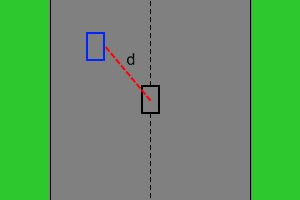
\includegraphics[width=0.7\textwidth]{fig/opendist.PNG}
		\label{fig}
		\begin{minipage}{10cm}
			\centering
			\caption{\footnotesize Trackpos sensor value.}
		\end{minipage} 
	\end{figure}
	\item \textbf{rpm:}  Number of rotation per minute of the car engine.
	\begin{figure}[h!]
		
		\centering
		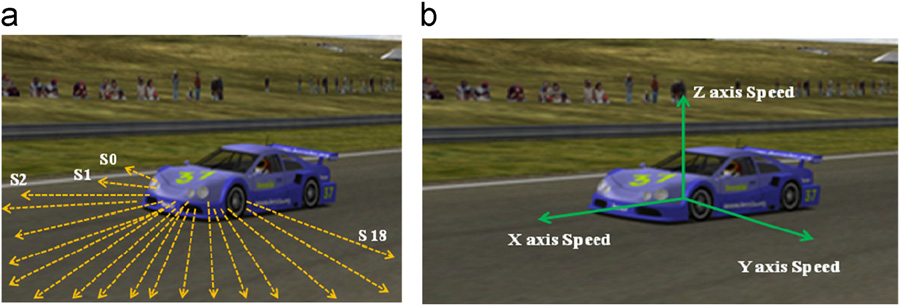
\includegraphics[width=0.9\textwidth]{fig/CARSEN.PNG}
		\begin{minipage}{10cm}
			\centering
			\caption{\footnotesize (a) Position sensor (b) Speed sensors.}
			\label{14}
		\end{minipage} 
	\end{figure}
	\newpage
	
	\item \textbf{speedX:} (km/h) Speed of the car along the longitudinal axis of the car.
	\item \textbf{speedY:} (km/h) Speed of the car along the transverse axis of the car.
	\item \textbf{speedZ:}  (km/h) Speed of the car along the Z axis of the car (See fig.\ref{14}).
	
	
	\item \textbf{track:}   
	
	Vector of 19 sensors each returns the distance between the edge of the track and the car within 100 meters. By default, the sensors sample the space in front of the car every 10 degrees, spanning clockwise from -90 degrees to +90 degrees to the axis of the car. However, the configuration of the track sensors can be set by the client once during initialization, before the start of each race. When the car is outside the track (less than -1 or greater than 1), the returned values are not reliable (usually -1 is returned).
	
	( See fig~\ref{tab16} and fig.\ref{14})
	\begin{figure}[h!]
		\centering
		\includegraphics[width=0.7\textwidth]{fig/Track.PNG}
		
		\begin{minipage}{10cm}
			\centering
			\caption{\footnotesize Track borders sensors.}
			\label{tab16}
		\end{minipage} 
		
		
	\end{figure}
	\newpage
	\item \textbf{trackPos:} 		
	Distance between the car and the axis of the track. The value is normalized to the width of the track: it is 0 when the car is on the axis, -1 when the car is on the right edge of the track and 1 when it's on the left. Values greater than 1 or less than -1 means that the car is outside the track[\cite{torcs2}](Voir fig\ref{tab17})
	\begin{figure}[h!]
		\centering
		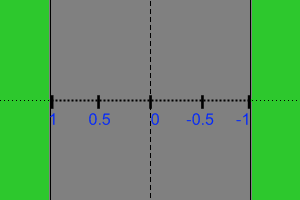
\includegraphics[width=0.7\textwidth]{fig/position.PNG}
		\begin{minipage}{10cm}
			\centering
			\caption{\footnotesize Car position in the race.}
			\label{tab17}
		\end{minipage} 

		
	\end{figure}
	
	
	\item \textbf{wheelSpinVel:}  Vector of 4 sensors representing the rotation speed of wheels.\\
	\item \textbf{Z:}  Distance of the car mass center from the surface of the track along the Z axis.
	
\end{enumerate}

\subsubsection{Actuators}

The driver bot is controlled in the game TORCS through a  typical set of actuators: the steering wheel "Steer", the accelerator "accel" the brake pedal and the gearbox. In addition, a meta-action is available to request a restart of the race to the server. Table~\ref{tab2}  details the available actions and their representation. [\cite {torcs} ]


\begin{table}[h!]
	
	\begin{tabular}{|p{3cm}|p{3 cm}|p{6 cm}|}
		\hline
		
		{\textbf{Action} }&
		{\textbf{Range} (unit)} &  
		{\textbf{Data type}}\\ 
		\hline
		Acceleration & [0,+1] & Double\\ 
		\hline
		Brake & [0,+1]	& Double\\
		\hline
		Gear & -1..0..+6	& Double\\
		\hline
		Steer & [-1,+1]	& Double\\
		\hline
		Clunch & [-1,+1]	& Double\\
		\hline
	\end{tabular}
	
	\caption{TORCS Effectors}
	\label{tab2}
\end{table}




\section{TORCS Controller Architecture}
The basic architecture of a controller consists of 5 simple modules (fig.\ref{archi}). This modular architecture  is a key factor to achieve good results. The basics modules functions  are explained below [\cite{fuzzy}]:

\begin{figure}[h!]
	
	\centering
	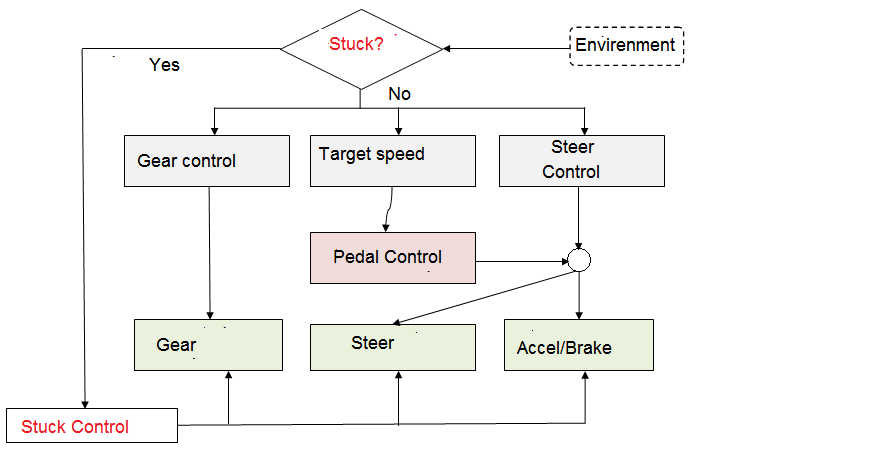
\includegraphics[width=0.9\textwidth]{fig/archicontrole2.PNG}
	\begin{minipage}{10cm}
		\centering
		\caption{\footnotesize Controller's Architecture.}
		\label{archi}
	\end{minipage} 	
\end{figure}
\newpage


\begin{enumerate}
	
	
	\item The gear control is mainly responsible for switching between first and sixth gear. Its functionality is completed with the task of detecting stuck  situations to apply the reverse.
	
	\item The target speed unit affects the speed limit for a track segment.
	
	\item speed control uses the results of others modules  to update or maintain certain speed by managing the throttle and the brake pedal. In addition, two techniques are implemented to prevent the car from slipping. A traction control (TCL) and an anti-lock anti-brake system (ABS) that will reduce, if necessary, actions over the accelerator and brake, respectively.
	
	\item Steer control module  manages the car's direction by acting on the vehicle wheel.[\cite{fuzzy}]
	\item The learning module detects segments of the track where the target speed can be increased or decreased with information on the previous laps, straight segments or segments where the car is off the track [\cite{fuzzy2}].
\end{enumerate}
\section{Simple driver}	
TORCS  comes with a simple driver often used to validate new designed controllers	 [\cite{torcs}][\cite{torcs2}]. \\
This project was provided by the TORCS software, and it was developed by \textit{Daniele Loiacono}  in 2007. It presents very basic functions for controlling the race car to give developers an idea of what the controller should look like. It contains simple functions to control the speed, steering angle and speed without dealing with opponents. Below are the driving principles in this system [\cite{torcs}]:\\

\begin{enumerate}
	
	
	\item 	If the car is at an angle that exceeds 30 degrees with the axis of the track  for at least 25 consecutive ticks, then it is considered in stuck.In this case, the simple driver sets the car in reverse with an angle which is the negative of the current angle. It drives the car that way at low speed until the front of the car is facing the border of the track. For example, if the car is on the left side, then it should be turned to the left. At that time, the car moves into first gear and the steering angle is reversed, so that the car can start moving forward again[\cite{torcs2}]. \\
	\item 	If the car is not in stuck, the simple driver proceeds as follows  [\cite{torcs2}]:\\
	\begin{itemize}
		\item 	First, it calculates the target speed. To do this, it gets the forward distance along the axis of the car by the front sensor FS and the sensor at 5 degrees to the left LS and 5 degrees to the right RS, as shown in Figure \ref {fig342}. Suppose RS> FS. Then, the driver made a first estimation of the "Steering angle" as the angle between the tangent to the road so that the car is facing the direction of car to the left else the angle is taken to the right. 
		
		\item Then, the target speed is calculated as follows
		
		\begin{equation}
		targetSpeed = \frac{(maxSpeed*FS*\sin(turnAngle))}{maxSpeedDist}
		\end{equation}	
		where: 	maxSpeed and maxSpeedDist are constant of the car.
		\begin{figure}[h!]
			
			\centering
			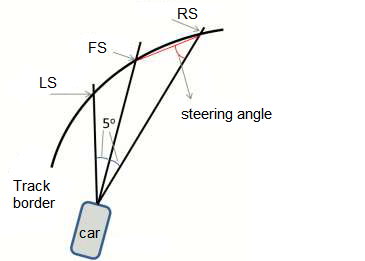
\includegraphics[width=0.7\textwidth]{fig/sensor02.PNG}
			\begin{minipage}{10cm}
				\centering
				\caption{\footnotesize Computing steering angle in simple driver.}
				\label{fig342}
			\end{minipage} 
		\end{figure}
	\end{itemize}		
	
\end{enumerate}
\section{Fuzzy based controllers design (AD1)}
%	\subsection{Conception de" AD" dans le cas sans adversaire}
The proposed controller "AD" has the same modular architecture as the simple driver where the target speed  and speed values are  computed via fuzzy controller using five 5 position sensors.

%	\subsubsection{{\color{red}Approche 1: Conception à l'aide des capteurs}}

%	\paragraph{- Structure du contrôleur floue pour calculer la vitesse cible\\\\}

\begin{figure}[h!]
	
	\centering
	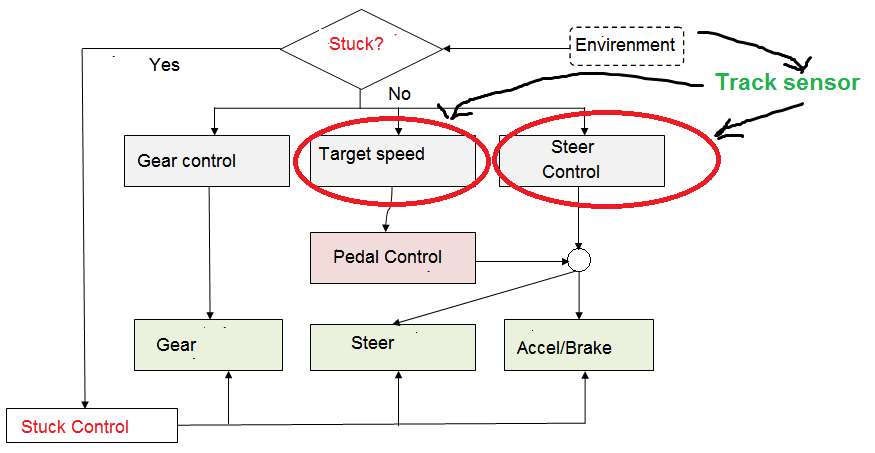
\includegraphics[width=0.8\textwidth]{fig/speedcible3.PNG}
	\begin{minipage}{10cm}
		\centering
		\caption{\footnotesize Target speed fuzzy control Architecture.}
		\label{archi2}
	\end{minipage} 
\end{figure}
\subsection{Fuzzy target speed}
To estimate the target speed  based on fuzzy rules, two cases are considered.
\begin{enumerate}
	\item If the car is in straight line, the target speed will take a maximum value (maxSpeed).\\\\
	\item If it is near a curve, the controller will decrease its current speed to a value included in the interval [minSpeed; maxSpeed] km / h for example if the turn is a strict turn the target speed will have a minimum value and a wide turn, it will have an average value.
	
\end{enumerate}
In case the car is off the track or near a curve, the brake system is activated, ie the ABS and TCS will be loaded to avoid the car skidding.
\\
The obtained target speed will be used in calculating the value of acceleration
(see fig.\ref{fig32} et fig.\ref{fig33}).
\\\\
\begin{equation}	
Gas(speed-Target_{speed})=-1+\frac{2}{1+e^{speed-Target_{speed}}}	
\end{equation}

Gas is for acceleration, Speed is the  current speed of the car.\\
Our fuzzy controller has 3 input values and one output: the target speed value(See figure \ref{AD}):

\begin{figure}
	\begin{center}
		
		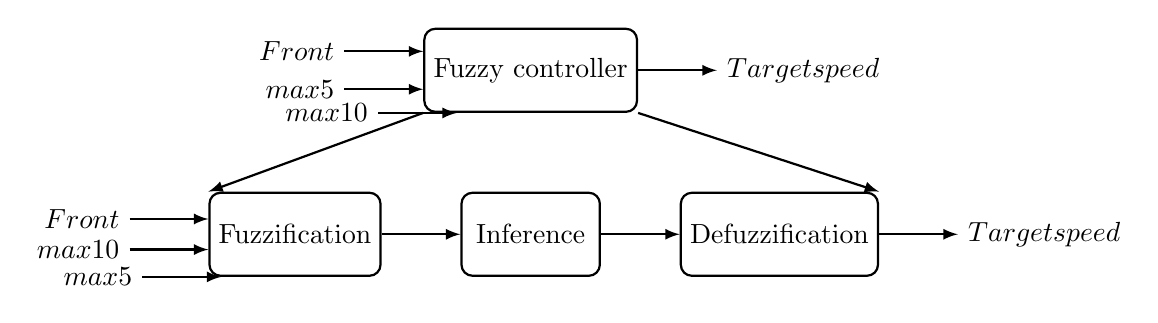
\begin{tikzpicture}[box/.style={draw, fill=white!20,rounded corners,align=center,minimum height=3em, minimum width=5em},thick,->,>= latex]
		
		\node[box] (a0) {Fuzzy controller};
		\node[left=of a0.170,font=\bfseries] (aux01) {$Front$};
		\node[left=of a0.190,font=\bfseries] (aux02) {$max 5$};
		\node[left=of a0.210,font=\bfseries] (aux03) {$max10 $};
		\node[right=of a0,font=\bfseries] (c0) {$Target speed$};
		\draw[thick,->,>= latex] (aux01) -- (a0.170);
		\draw[thick,->,>= latex] (aux02) -- (a0.190);
		\draw[thick,->,>= latex] (aux03) -- (a0.210);
		\draw[thick,->,>= latex] (a0) -- (c0);
		\node[box,below=of a0] (b) {Inference};
		
		\node[box, left=of b] (a) {Fuzzification};
		\node[left=of a.170,font=\bfseries] (aux1) {$Front$};
		\node[left=of a.190,font=\bfseries] (aux2) {$max10$};
		\node[left=of a.210,font=\bfseries] (aux3) {$max 5$};
		
		\node[box,right=of b] (b1) {Defuzzification};
		\node[right=of b1,font=\bfseries] (c) {$Target speed$};
		\draw[thick,->,>= latex] (aux1) -- (a.170);
		\draw[thick,->,>= latex] (aux2) -- (a.190);
		\draw[thick,->,>= latex] (aux3) -- (a.210);
		\draw[thick,->,>= latex] (a) -- (b);
		\draw[thick,->,>= latex] (b) -- (b1);
		\draw[thick,->,>= latex] (b1) -- (c);
		
		
		\draw[thick,->,>= latex] (a0.south west) -- (a.north west);
		\draw[thick,->,>= latex] (a0.south east) -- (b1.north east);
		
		
		\end{tikzpicture}
		
		%\includegraphics [width=10cm,height=4cm]{figures/c2/sif}
	\end{center}
	\caption{Fuzzy control of target speed.}     % width is 8.4 cm.
	\label{AD}
\end{figure}



The "AD" controller is a Mamdani based fuzzy system (See fig.\ref{AD}) with trapezoidal membership functions for input variables. It uses three values among the 19 of the track sensor (See fig.\ref{fig34}):\\

\begin{enumerate}
	\item Front = Track[9]  with angle = 0 , the front distance between the car and the border of track.
	\item max5 = max (Track[8]; Track[10])
	the max distance with +5 and  -5 angle.
	\item max10 = max (track[11]; track[7]) ,	the max distance with +10 and  -10 angle.
\end{enumerate}
\begin{figure}[h!]
	
	\centering
	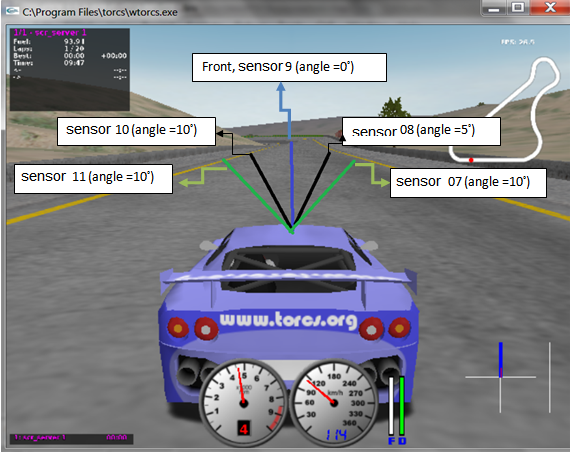
\includegraphics[width=0.9\textwidth]{fig/sensor22.PNG}
	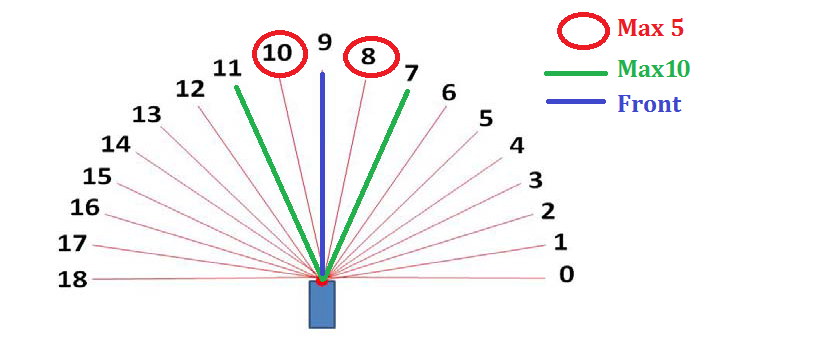
\includegraphics[width=0.9\textwidth]{fig/front.PNG}
	\begin{minipage}{10cm}
		\centering
		\caption{\footnotesize Fuzzy inputs.}
		\label{fig34}
	\end{minipage} 		
\end{figure}
\newpage
\begin{enumerate}
	
	\item{\textbf{Fuzzification}}
	
	Each input variable is represented by three membership functions Low, Medium
	and High as shown in the figures (fig. \ref {forehead} , Fig. \ref{max5} , fig, \ref{max15} , Fig. \ref{fontfig})\\
	The description of fuzzy inputs and output are represented in table \ref{flouevar} .\\	
	
	\begin{table} [h!] 
		\label{flouevar}
		\caption{ Fuzzy variables description}
		\begin{tabular}{ |p{1cm}|p{2cm}|p{1.5cm}|p{2 cm}|p{1 cm}|p{1.5 cm}|p{1.5 cm}|}
			\hline
			{ \color{red} Variable }&
			{ \color{red}Range }&
			{ \color{red}Name}&  
			{ \color{red} MF } &
			{ \color{red} Low } &
			{ \color{red} Medium }&
			{ \color{red} High } 
			
			\\
			\hline
			Input & [0-100] m & Front & trapezoidal & [0-50] & [20-80] &[80-100]
			\\
			\hline
			Input & [0-100] m & max 5 & trapezoidal &[0-40] & [10-70] & [40-100] 
			\\
			\hline
			Input & [0-100] m  & max 10 & trapezoidal & [0-30] & [0-60] & [30-100]
			\\
			\hline 
			Output & [0-200]m/s & TS & singleton & / & / & /
			\\
			\hline 
		\end{tabular} 
	\end{table}
	\begin{figure}
		\begin{center}
			
			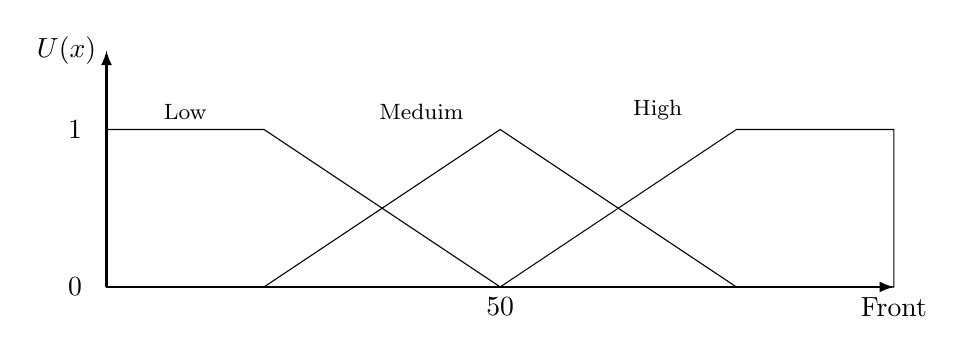
\begin{tikzpicture}[scale=2]
			%\draw[->] (0,0) -- node[below] {quantized} (4.5,0) node[below] {Age};
			%\draw[->] (0,0) -- (0,1.5) node[left] {$\mu$};
			%\node at (-0.2,0) {0};
			%\node at (-0.2,1) {1};
			%\draw[fill=yellow] (0,1) -- (4,1) -- (4,0) -- (0,0) -- cycle;
			%\foreach \x in {0.5,1,1.5,2,2.2,3.4}
			%  \draw (\x,0) -- (\x,1);
			\begin{scope}[xshift=2cm]
			\draw[thick,->,>= latex] (0,0) -- node[below] {50} (5,0) node[below] {Front};
			\draw[thick,->,>= latex] (0,0) -- (0,1.5) node[left] {$U(x)$};
			\node at (-0.2,0) {0};
			\node at (-0.2,1) {1};
			\draw (0,1) -- (1,1) -- (2.5,0) -- (0,0) -- cycle;
			\draw (1,0) -- (2.5,1) -- (2.5,1) -- (4,0) -- cycle;
			\draw (2.5,0) -- (4,1) -- (4,1) -- (5,1) -- (5,0) -- cycle;
			
			%\draw[fill=blue!40] (2.25,0) -- (3,1) -- (4,1) -- (4,0) -- cycle;
			%\draw[fill=blue!40] (1.25,0) -- (1.8,1) -- (2.3,1) -- (3,0) -- cycle;
			%\draw (1,1) -- (1.75,0) -- (2.25,0) -- (3,1);
			\node[above,font=\footnotesize] at (0.5,1) {Low};
			\node[above,font=\footnotesize] at (2,1) {Meduim};
			\node[above,font=\footnotesize] at (3.5,1) {High};
			\end{scope}
			%\node[anchor=south] at (current bounding box.north)
			%  {\textbullet\ continuous $\rightarrow$ quantized $\rightarrow$ granulated};
			\end{tikzpicture}
			%\includegraphics [width=10cm,height=4cm]{figures/c2/exemple_floue}
		\end{center}
		\caption{Membership functions of  "Front".}     % width is 8.4 cm.
		\label{front}
	\end{figure}
	\begin{figure}
		\begin{center}
			
			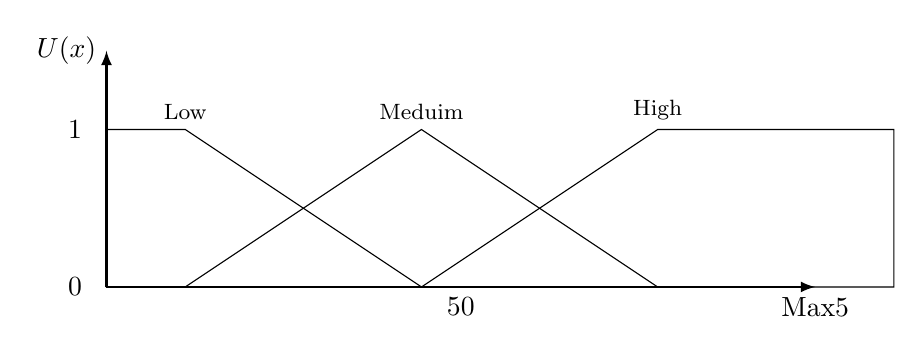
\begin{tikzpicture}[scale=2]
			%\draw[->] (0,0) -- node[below] {quantized} (4.5,0) node[below] {Age};
			%\draw[->] (0,0) -- (0,1.5) node[left] {$\mu$};
			%\node at (-0.2,0) {0};
			%\node at (-0.2,1) {1};
			%\draw[fill=yellow] (0,1) -- (4,1) -- (4,0) -- (0,0) -- cycle;
			%\foreach \x in {0.5,1,1.5,2,2.2,3.4}
			%  \draw (\x,0) -- (\x,1);
			\begin{scope}[xshift=2cm]
			\draw[thick,->,>= latex] (0,0) -- node[below] {50} (4.5,0) node[below] {Max5};
			\draw[thick,->,>= latex] (0,0) -- (0,1.5) node[left] {$U(x)$};
			\node at (-0.2,0) {0};
			\node at (-0.2,1) {1};
			\draw (0,1) -- (0.5,1) -- (2,0) -- (0,0) -- cycle;
			\draw (0.5,0) -- (2,1) -- (2,1) -- (3.5,0) -- cycle;
			\draw (2,0) -- (3.5,1) -- (3.5,1) -- (5,1) -- (5,0) -- cycle;
			\node[above,font=\footnotesize] at (0.5,1) {Low};
			\node[above,font=\footnotesize] at (2,1) {Meduim};
			\node[above,font=\footnotesize] at (3.5,1) {High};
			\end{scope}
			%\node[anchor=south] at (current bounding box.north)
			%  {\textbullet\ continuous $\rightarrow$ quantized $\rightarrow$ granulated};
			\end{tikzpicture}
			%\includegraphics [width=10cm,height=4cm]{figures/c2/exemple_floue}
		\end{center}
		\caption{Membership functions of  "Max5".}     % width is 8.4 cm.
		\label{max5}
	\end{figure}
	\begin{figure}
		\begin{center}
			
			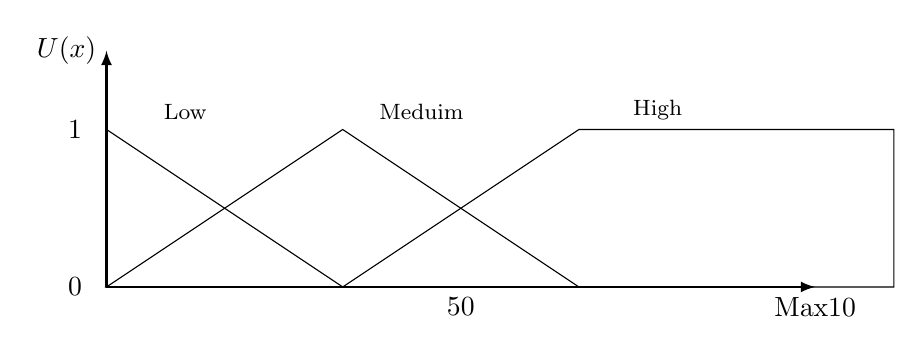
\begin{tikzpicture}[scale=2]
			%\draw[->] (0,0) -- node[below] {quantized} (4.5,0) node[below] {Age};
			%\draw[->] (0,0) -- (0,1.5) node[left] {$\mu$};
			%\node at (-0.2,0) {0};
			%\node at (-0.2,1) {1};
			%\draw[fill=yellow] (0,1) -- (4,1) -- (4,0) -- (0,0) -- cycle;
			%\foreach \x in {0.5,1,1.5,2,2.2,3.4}
			%  \draw (\x,0) -- (\x,1);
			\begin{scope}[xshift=2cm]
			\draw[thick,->,>= latex] (0,0) -- node[below] {50} (4.5,0) node[below] {Max10};
			\draw[thick,->,>= latex] (0,0) -- (0,1.5) node[left] {$U(x)$};
			\node at (-0.2,0) {0};
			\node at (-0.2,1) {1};
			\draw (0,1) -- (0,1) -- (1.5,0) -- (0,0) -- cycle;
			\draw (0,0) -- (1.5,1) -- (1.5,1) -- (3,0) -- cycle;
			\draw (1.5,0) -- (3,1) -- (3,1) -- (5,1) -- (5,0) -- cycle;
			\node[above,font=\footnotesize] at (0.5,1) {Low};
			\node[above,font=\footnotesize] at (2,1) {Meduim};
			\node[above,font=\footnotesize] at (3.5,1) {High};
			\end{scope}
			%\node[anchor=south] at (current bounding box.north)
			%  {\textbullet\ continuous $\rightarrow$ quantized $\rightarrow$ granulated};
			\end{tikzpicture}
			%\includegraphics [width=10cm,height=4cm]{figures/c2/exemple_floue}
		\end{center}
		\caption{Membership functions of  "Max10".}     % width is 8.4 cm.
		\label{max15}
	\end{figure}
	
	\begin{figure}[h!]
		
		\centering
		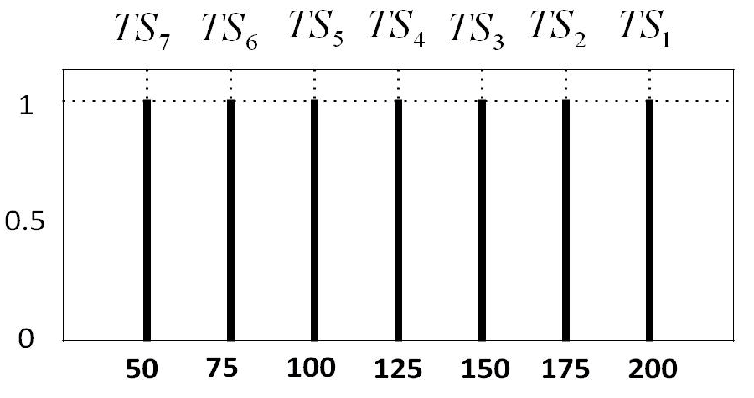
\includegraphics[width=0.7\textwidth]{fig/speed.PNG}
		\begin{minipage}{10cm}
			\centering
			\caption{\footnotesize Target speed values.}
			\label{fontfig}
		\end{minipage} 
		\index{tracé}                     %% inclure le mot tracé dans l'index
		\index{fonction}                  %% include le mot fonction dans l'index
		
	\end{figure}
	
	\item{\textbf{Fuzzy inference system}}
	The rules base is designed on the principle that if the front distance is maximal, then target speed should be maximal, and this value should be less when  the frontal distance is lower. The fuzzy rules are listed below:
	\\
	\begin{enumerate}
		
		
		\item If Front is High Then TargetSpeed is TS1
		\item If Front is Medium Then TargetSpeed is TS2
		\item If Front is Low and Max5 is High Then TargetSpeed is TS3
		\item If Front is Low and Max5 is Medium Then TargetSpeed is TS4
		\item If Front is Low and Max5 is Low and Max10 is High Then TargetSpeed is TS5
		\item If Front is Low and Max5 is Low and Max10 is Medium Then TargetSpeed is TS6
		\item  If Front is Low and Max5 is Low and Max10 is Low Then TargetSpeed is TS7
		\\
		In addition, a crisp rule is added to rule base to obtain a maximum value of a target speed when the value of the three input variables as far as possible, less than 100 m: \\\\
		\item If Front = Maxdistspeed or Max5 = Maxdistspeed or Max10 = Maxdistspeed Then TargetSpeed = Maxspeed	
		
	\end{enumerate}
	
	\item{\textbf{Deffuzzification}}
	The output value (target speed) is encoded by seven singletons.
	This phase is to transform the fuzzy set of output in a real value for the controlled system . \\
	
	\subsection{Fuzzy Steer}
	
	We can use another fuzzy controller in the control of the Steer to estimate and determine the target position of the car:\\
	if the car is straight line then it will take as target position half width of the race track.\\
	
	
	\begin{figure}[h!]
		
		\centering
		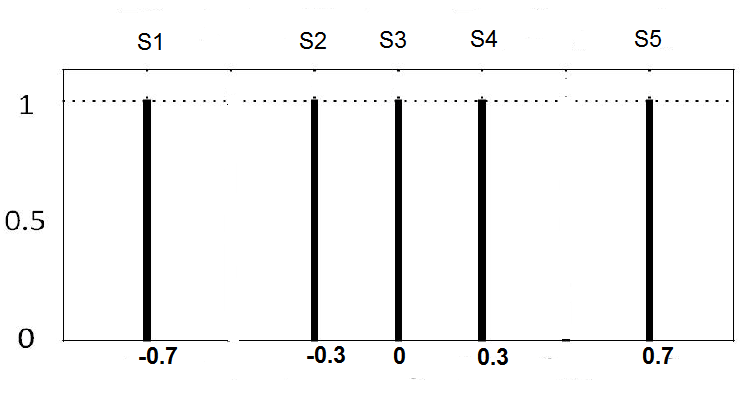
\includegraphics[width=0.4\textwidth]{fig/speed2.PNG}
		\begin{minipage}{10cm}
			\centering
			\caption{\footnotesize Steer values.}
			\label{fontfig6}
		\end{minipage} 
	\end{figure}
	
	
	
	If the car is near a right curve,it will approach the path leading to the right, with a space between the car and the border of the track to avoid the loss of control and shocks .The same if the car is near a left curve (see fig. \ref {steercont} ) \\
	
	Detection of curves is based on the sensor values (max10, max5, front).
	
	\begin{figure}[h!]
		
		\centering
		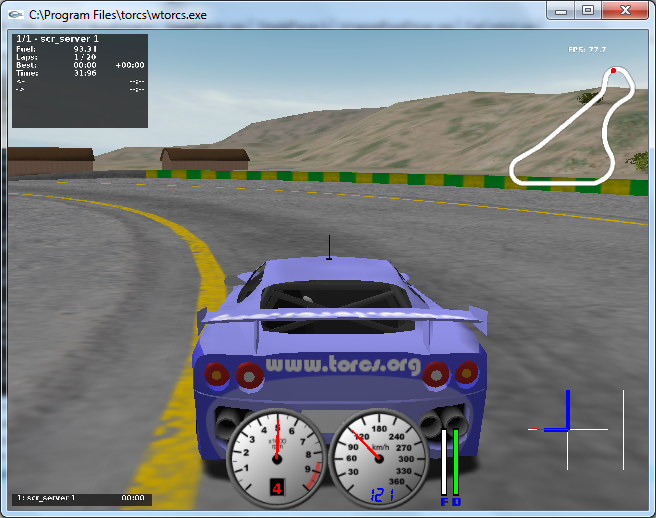
\includegraphics[width=0.5\textwidth]{fig/steercont.PNG}
		\begin{minipage}{10cm}
			\centering
			\caption{\footnotesize 'Steer control' of a car in a curve.}
			\label{steercont}
		\end{minipage} 
	\end{figure}
	the rule base is presented as follows:\\
	\begin{itemize}
		
		\item If Front is High Then steer is S3
		\item If Front is Medium Then steer is TS2
		\item If Front is Low and Max5 is High Then steer is TS3
		\item If Front is Low and Max5 is Medium Then steer is TS4
		\item If Front is Low and Max5 is Low and Max10 is High Then steer is TS5
		\item If Front is Low and Max5 is Low and Max10 is Medium Then steer is TS6
		\item  If Front is Low and Max5 is Low and Max10 is Low Then steer is TS7
		\\
	\end{itemize}	
\end{enumerate}	
\section{{\color{red}Turning Radius based fuzzy control (AD3) }}


In this section, we focus on controlling the direction of the car "Steer control" and control of the target speed using the turning radius.
\begin{figure}[h!]
	
	\centering
	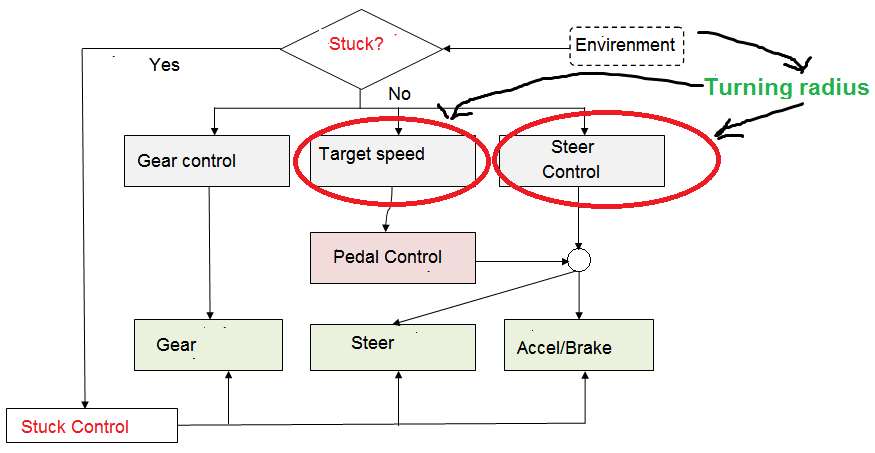
\includegraphics[width=0.7\textwidth]{fig/steercible3.PNG}
	\begin{minipage}{10cm}
		\centering
		\caption{\footnotesize Turning radius fuzzy control architecture.}
		\label{fig45}
	\end{minipage} 
\end{figure}
\subsection{Car Turning geometry }	
There are many techniques used to turn a car, but the most effective one is to study the geometry of the driving line of the car and the geometry of the track such as detecting track borders ... \\

Three cases are considered in control of the wheel (see equation (3) and (4)) \\

\begin{equation}
Steer =  angle - 0.5 *\frac{position }{Steer_lock}		
\end{equation}

\begin{equation}
Steer =  \frac{angle }{Steer_lock}	
\end{equation}

$SteerLock $ is a constant value  from the description available in TORCS of the car  and its value is 0.785		
\begin{enumerate}
	\item  The car is inside the track, it takes a restrained line \\
	\item  The car is outside of the track, the system initiates the stuck control function.\\
	\item  The car is near a curve to the right or left, we study the turning geometry. \\	
\end{enumerate}	


\subsubsection{turning geometry}
The turning radius is the minimum radius of the circle described by a car during a turn. His goal in our case is to have the target position when the car is a curve. (See fig. \ref {fig09})
\begin{figure}[h!]
	
	\centering
	\includegraphics[width=0.4\textwidth]{fig/rayon.PNG}
	\includegraphics[width=0.2\textwidth]{fig/06.PNG}
	
	%\includegraphics[width=0.8\textwidth]{salm.PNG}
	
	
	\begin{minipage}{10cm}
		\centering
		\caption{\footnotesize Turning radius.}
		\label{fig09}
	\end{minipage} 
\end{figure}


Figure \ref {fig04} represents the path of the turn (right / left), it is cut into 4 parts-such as:
\begin{enumerate}
	\item  The entrance area (Blue):\\
	its goal is to put the car near the centre line and to determine a braking point when the sensors show that the turn is not far away. (See \ref {fig05})
	
	\item discovery area (Green).\\
	Here, while keeping the car close to the center line and starting to register curve, will, look, go for a sign which materializes the end of the turn.\\
	The acceleration must remain constant and the same as from the entrance. (See Fig \ref {fig05})
	\item Solicitation area (red).\\		
	Here, the driver starts to determine the inside turning radius. (See Fig \ref {fig05})
	\item Stability recovering area (yellow)\\
	The car is gets outside the curve. In fact, in this area, the car straightens and we leave to the next turn.
\end{enumerate}
\begin{figure}[h!]
	\centering
	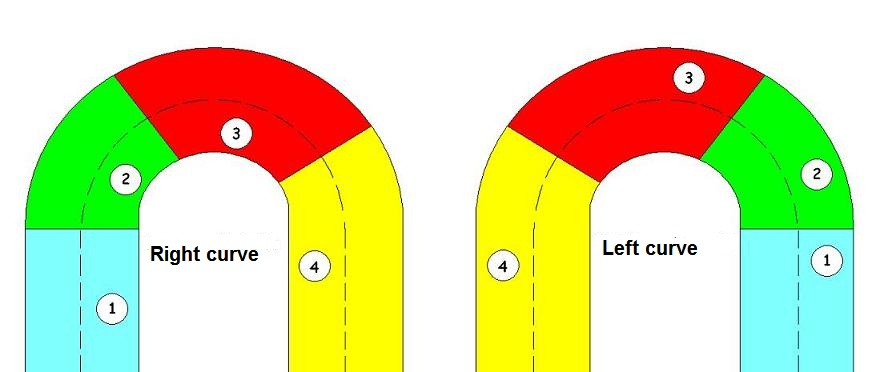
\includegraphics[width=0.7\textwidth]{fig/virage.PNG}
	\begin{minipage}{10cm}
		\centering
		\caption{\footnotesize Right and left curves.}
		\label{fig04}
	\end{minipage} 
	
\end{figure}

The curve used is a circle see Figure \ref {fig05}, in order to have a single look point (the target) possible.
The coordinates are given relative to the car centre. \\	

\begin{figure}[h!]
	
	\centering
	%	\includegraphics[width=0.9\textwidth]{06.PNG}
	%	\includegraphics[width=0.5\textwidth]{rayon.PNG}
	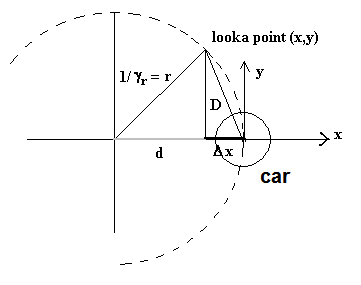
\includegraphics[width=0.9\textwidth]{fig/salm2.PNG}
	
	
	\begin{minipage}{10cm}
		\centering
		\caption{\footnotesize Turning radius.}
		\label{fig05}
	\end{minipage} 
	
\end{figure}

The Y axis: the axis is formed by the straight line passing through the middle of the car in the direction of movement \\.	
The X axis passes through the middle of the vehicle perpendicular to the direction of movement to the right \\.

(xr, yr) is the current position of the vehicle, and (xg, yg) is the target to be  converted the vehicle mark.

\begin{gather}
xgv = (xg - xr)\cos(\theta)+ (yg-yr)\sin(\theta)\\
ygv = -(xg - xr)\sin(\theta) + (yg-yr)\cos(\theta).
\end{gather}
Where (xgv, ygv) are the coordinates of the target in the vehicle mark and $\theta $ is the current direction of the car.\\
D is the distance between the centre of the vehicle and the target.  $1 /\gamma$ is the radius of the circle that pass through the centre of the car and the target.
The curvature of the vehicle's trajectory path is calculated as follows:
\begin{equation}	
\gamma r = 2\delta x/D^2		
\end{equation}
This equation is obtained using the following equations:
\begin{gather}
x^2 + y^2 = D^2	\\
x + d = r  
\end{gather}

(x,y) are the target coordinates. We have:\\
\begin{gather}
d = r - x\\
(r - x)^2 + y^2 = r^2  \\
r^2 - 2rx + x^2 + y^2 = r^2\\	
2rx = D^2\\	
r = D^2/2x\\
\gamma r = 2x/D^2\\
\end{gather}	

\subsection{Turning radius based Fuzzy controller design}
Now it is easy to set up the architecture of our fuzzy controller to determine the target position of the car (see Figure \ref {fig36}). We will have two fuzzy controllers with the same input, one is for the target position and the other is for the target speed. 
\begin{figure}[h!]
	
	\centering
	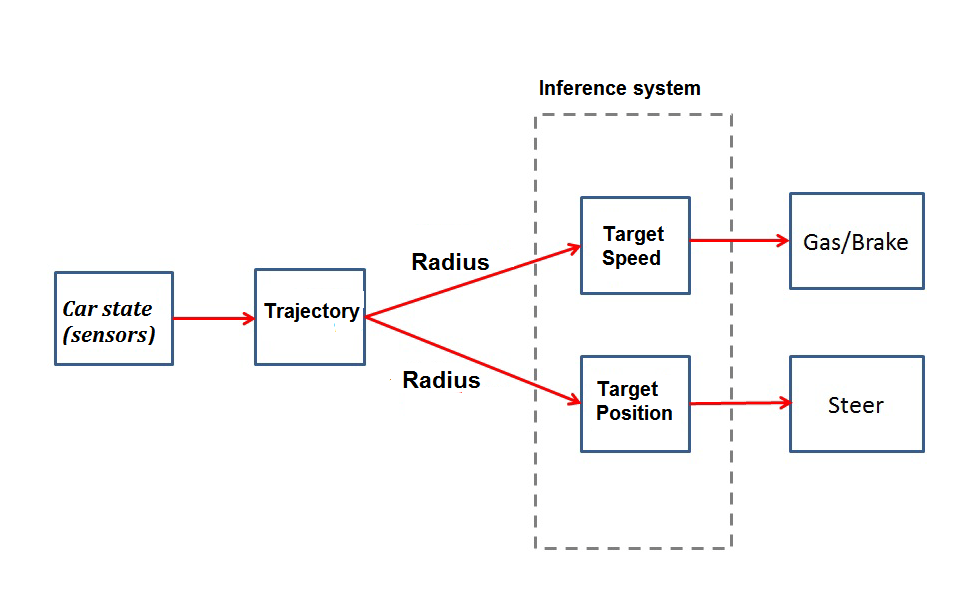
\includegraphics[width=0.9\textwidth]{fig/rayon21.PNG}
	\begin{minipage}{10cm}
		\centering
		\caption{\footnotesize Fuzzy controller Structure.}
		\label{fig36}
	\end{minipage} 
	
\end{figure}

\subsubsection{Fuzzyfication}

In our case we have real input for the two fuzzy controllers which is the turning radius R and as output "The target position TP  for the first one and the target speed TS  for the other one .(Table \ref{fig39}) (see Figure \ref{fig37} \ref{fig38})

\begin{table} [h!] 
	\label{fig39}
	\caption{ Fuzzy controllers description}
	\begin{tabular}{ |p{4.5cm}|p{3cm}|p{3cm}|p{3cm}|}
		\hline
		&{ \color{red} Radius  }&
		{\color{red}TP }&
		{\color{red}TS }\\
		\hline
		
		{ \color{red} Type }& Input & Output first FC & Output of second FC\\
		\hline
		{ \color{red}Ranges}&[0-250] m&[0,1]m& [0-120]km/h\\
		
		\hline
		{ \color{red}fuzzy variable floue}& Radius & TP& TS
		\\
		\hline  
		{ \color{red} Membership functions} & trapezoidal  & singleton & singleton
		\\
		\hline
		{ \color{red} SEF "Low" } &   [0-125] & ----- & ------
		\\
		\hline
		{ \color{red} SEF "Medium" }&[50-200] & ----- & ------
		\\
		\hline
		{ \color{red} SEF "High" }  &[125-250]& ----- & ------
		\\
		\hline
		
		
		
		
	\end{tabular} 
\end{table}
\begin{figure}
	\begin{center}
		
		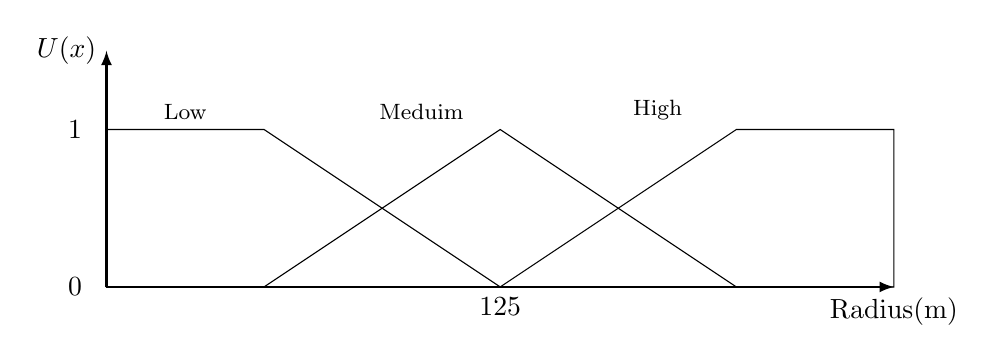
\begin{tikzpicture}[scale=2]
		%\draw[->] (0,0) -- node[below] {quantized} (4.5,0) node[below] {Age};
		%\draw[->] (0,0) -- (0,1.5) node[left] {$\mu$};
		%\node at (-0.2,0) {0};
		%\node at (-0.2,1) {1};
		%\draw[fill=yellow] (0,1) -- (4,1) -- (4,0) -- (0,0) -- cycle;
		%\foreach \x in {0.5,1,1.5,2,2.2,3.4}
		%  \draw (\x,0) -- (\x,1);
		\begin{scope}[xshift=2cm]
		\draw[thick,->,>= latex] (0,0) -- node[below] {125} (5,0) node[below] {Radius(m)};
		\draw[thick,->,>= latex] (0,0) -- (0,1.5) node[left] {$U(x)$};
		\node at (-0.2,0) {0};
		\node at (-0.2,1) {1};
		\draw (0,1) -- (1,1) -- (2.5,0) -- (0,0) -- cycle;
		\draw (1,0) -- (2.5,1) -- (2.5,1) -- (4,0) -- cycle;
		\draw (2.5,0) -- (4,1) -- (4,1) -- (5,1) -- (5,0) -- cycle;
		
		%\draw[fill=blue!40] (2.25,0) -- (3,1) -- (4,1) -- (4,0) -- cycle;
		%\draw[fill=blue!40] (1.25,0) -- (1.8,1) -- (2.3,1) -- (3,0) -- cycle;
		%\draw (1,1) -- (1.75,0) -- (2.25,0) -- (3,1);
		\node[above,font=\footnotesize] at (0.5,1) {Low};
		\node[above,font=\footnotesize] at (2,1) {Meduim};
		\node[above,font=\footnotesize] at (3.5,1) {High};
		\end{scope}
		%\node[anchor=south] at (current bounding box.north)
		%  {\textbullet\ continuous $\rightarrow$ quantized $\rightarrow$ granulated};
		\end{tikzpicture}
		%\includegraphics [width=10cm,height=4cm]{figures/c2/exemple_floue}
	\end{center}
	\caption{Membership function of the input: radius.}     % width is 8.4 cm.
	\label{fig37}
\end{figure}
\begin{figure}[h!]
	
	\centering
	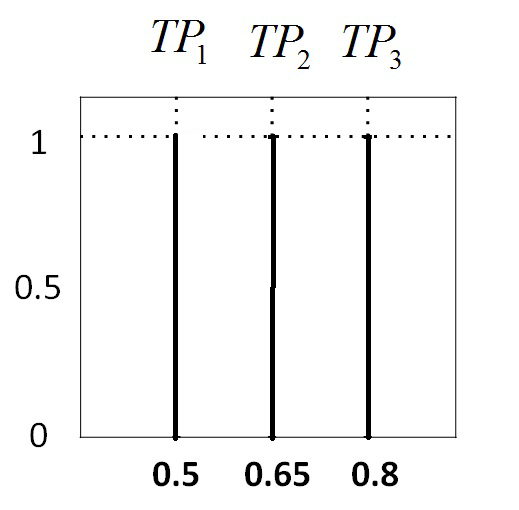
\includegraphics[width=0.4\textwidth]{fig/dis.PNG}
	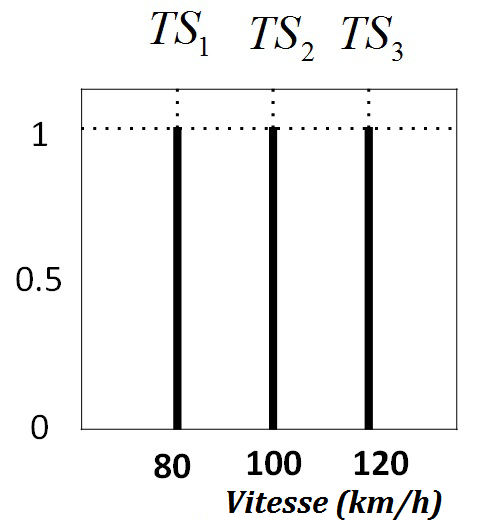
\includegraphics[width=0.34\textwidth]{fig/speed1.PNG}
	\begin{minipage}{10cm}
		\centering
		\caption{\footnotesize Membership function of the outputs: TP and TS.}
		\label{fig38}
	\end{minipage} 
	
\end{figure}
\subsubsection{Fuzzy inference}
The rules basis is designed on the principle that if the turning radius is equal to a very minimum then not turn so we will adjust the position of the car to the middle of the track, \\
otherwise if the turning radius is equal to a maximum value, so the position of the car will change its direction to the rotation path (right or left). (See Fig. \ref {fig04}) \\
And the same thing if the turning radius is equal to an average value, so we will approximate the rotation path (see Fig. \ref{fig04}) \\
This concept can also be applied to the estimated target speed \\

\begin{figure}[h!]
	
	\centering
	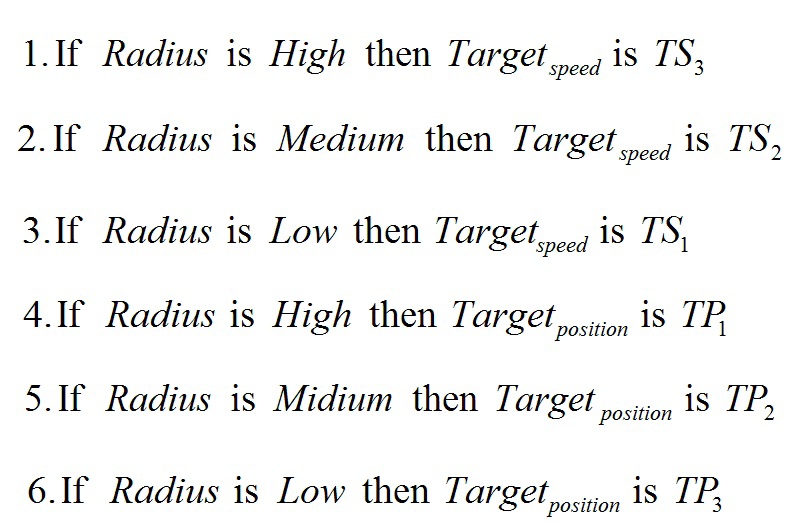
\includegraphics[width=0.6\textwidth]{fig/regle.PNG}
	\begin{minipage}{10cm}
		\centering
		\caption{\footnotesize Rule base of radius based fuzzy  controller .}
		\label{fig40}
	\end{minipage} 
	
	
\end{figure}

\subsection{AD5 fuzzy controller design}


The AD5 controller is a speed-steer based fuzzy controller with opponents consideration.\\

Using the previous approaches, we will adapt the driving behavior when opponents are nearby. It will modify or replace the outputs obtained from the steering, throttle and brake controllers.
\\

The modification of throttle control outputs, brake and steering will be mainly using information from opponents sensors .



Three types of updates are performed:
\begin{enumerate}
	
	\item on the steering output to avoid opponents (on hold)
	\item on the steer, but with a strong movement in the collision risk  (collision avoidance)
	\item the brake value when there is an adversary
	front of the car in a dangerous distance. \\
	Both actions on the steer are performed simultaneously.
	
\end{enumerate}
\begin{figure}[h!]
	
	\centering
	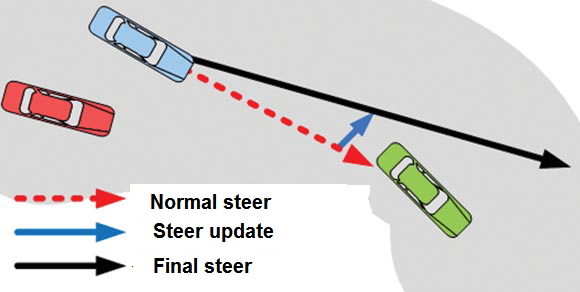
\includegraphics[width=0.6\textwidth]{fig/op.PNG}
	\begin{minipage}{10cm}
		\centering
		\caption{\footnotesize Car behaviour when opponent is nearby} 
		\label{fig42}
	\end{minipage} 
	
\end{figure}

\section{Simulation results}

In this section we present all the experiments that we performed in order to measure the performance of our controller "AD" (Algerian Driver) after developing many functions and adding many features.
We first describe the methodology we have used and next, we present the experimental results of the implementation of the "AD", with opponents and
using special criteria in each case. \\


We have established a set of tests to measure the performance of the controller "AD". We compared the newly developed Controller with existing methods: the single driver. We will run every single control car by choosing the car called "SRC-server1" in several race tracks. \\

\subsection{Simulation settings}

\subsubsection{Tracks settings}

TORCS provides different tracks to choose from. These race tracks are designed by different developers in order to test the performance of the controllers on different difficulty circuits and on different types of roads.\\

The TORCS training environment provides three main tracks: Road tracks, dirt tracks and oval tracks.
There are 21 tracks which are circuits of a substantial length with many curves of different difficulty. In addition, the system offers 8 dirt tracks, also very long and represents a growing challenge in terms of control of the car. There are 9 oval tracks, which are shorter and more predictable, and designed primarily to optimize speed.

During competitions, drivers can expect to be exposed to unfamiliar roads to challenge their ability to win the race with minimum damages in record time.\\

In our case, we chose three of road tracks, a dirt road, and an oval track.\\


On oval tracks, E-Track5 seems to be the most interesting, as it has curves in both directions. On dirt roads, Dirt1 has a good variety of curves. For road tracks, we selected three tracks: Forza, E-Road and CG-Speedway Number1. Table \ref{Tabtrack}  presents the properties and description of each selected track.\\

\begin{table}[h!]
	
	\caption{Description of Selected tracks}
	\label{Tabtrack}
	\begin{tabular}{ |p{2cm}|p{2 cm}|p{2 cm}|p{2 cm}|p{2 cm}|p{2 cm}|}
		\hline
		\textbf{Track name}    & E-Track5
		& Dir1 4 
		& Forza
		& E-Road
		& CG-Speedway Number1
		\\
		\hline
		\textbf{Shape}   
		& fig.\ref{fig3} (4)
		& fig.\ref{fig3} (2)
		& fig.\ref{fig3} (3) 
		& fig.\ref{fig3} (2)
		& fig.\ref{fig3} (1)
		
		\\
		\hline
		\textbf{Track Type}   
		& Oval
		& Dirty
		& Road
		& Road
		& Road
		
		\\
		\hline
		\textbf{Description}   
		& simple track race
		
		& Track for outdoor race
		& Very fast and smooth
		& Track race
		& rhythmic track and fast enough
		
		\\
		\hline
		
		\textbf{Length}   
		& 1621.73 m
		& 3260.43 m
		& 5784.10 m
		& 3260.43 m
		& 2057.56 m
		
		\\
		\hline
		\textbf{Width}   
		& 20.0 m
		& 16.0 m
		& 11.0 m
		& 16.0 m
		& 15.0 m
		\\
		\hline
	\end{tabular} 
\end{table}
\begin{figure}[h!]
	
	\centering
	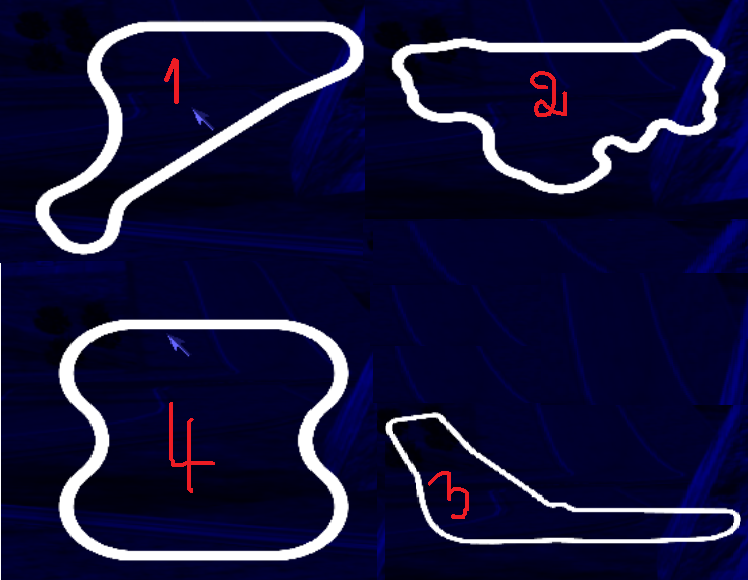
\includegraphics[width=0.7\textwidth]{fig/trackresultat.PNG}
	\begin{minipage}{10cm}
		\centering
		\caption{\footnotesize Tracks shape.}
		\label{fig3}
	\end{minipage} 
	
\end{figure}

\begin{figure}[h!]
	
	\centering
	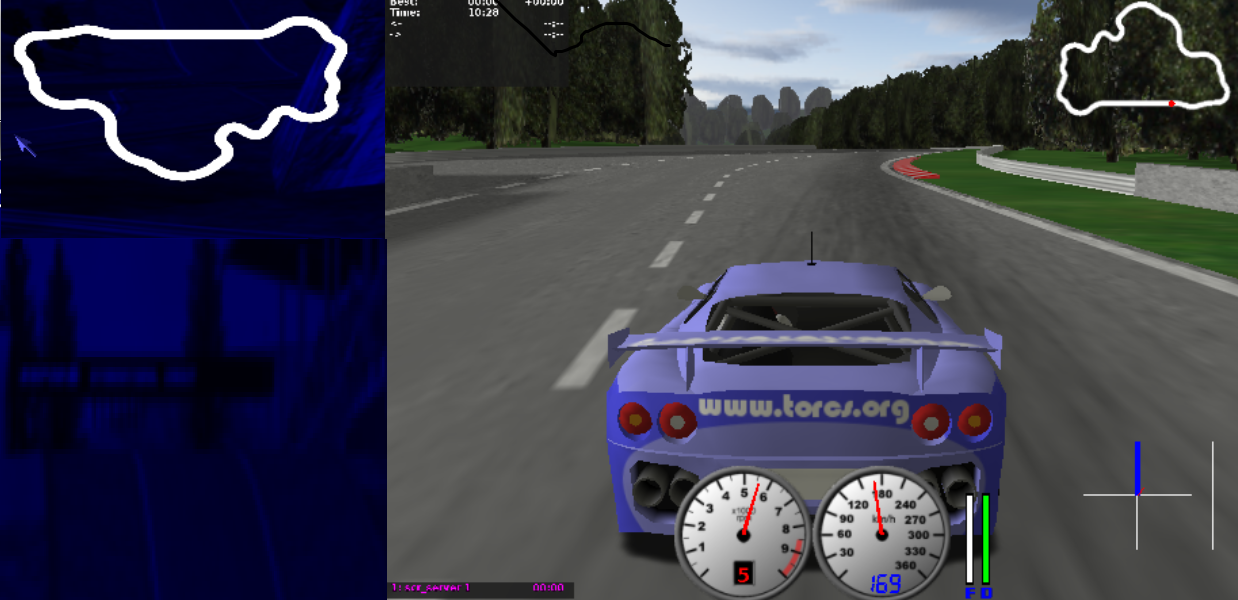
\includegraphics[width=0.8\textwidth]{fig/Eroad.PNG}
	\begin{minipage}{10cm}
		\centering
		\caption{\footnotesize A car in E-Road track.}
		\label{fig30}
	\end{minipage} 
	
\end{figure}
As Figure \ref{fig30} shows, the E-Road track is a road track with many curves of all kinds: fast, medium and slow curves. It allows us to test the performance more effectively.


\subsubsection{ Cars settings}

SCR 1 server is a NASCAR car and member of the SCR Server team (A team can used different types of car as  car1-stock1, car1-tbr1 ...).\\
A Sprint Cup Series NASCAR-type car weighs at least 1542 kg for 850 horses with . The engine is a V8 with  $ 5,866 cm ^ 3 $. Its chassis is tubular type. It has a Borg-Warner gearbox with four-speed for road circuits.\\

In our simulations, we used the car "car1-tbr1" see Fig.\ref{car} 
\begin{figure}[h!]
	
	\centering
	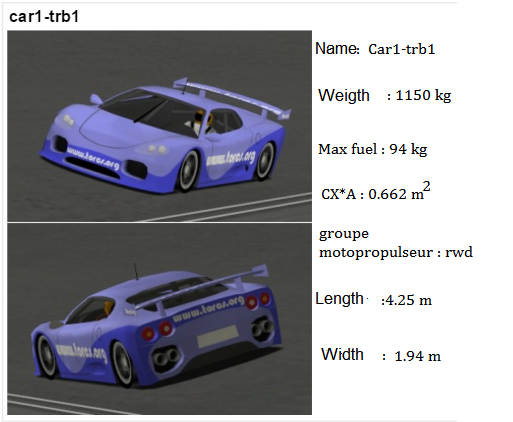
\includegraphics[width=0.8\textwidth]{fig/car1.PNG}
	\begin{minipage}{10cm}
		\centering
		\caption{\footnotesize car1-trb1 features  .}
		\label{car}
	\end{minipage} 
	
\end{figure}

\subsubsection{Controllers settings}
To validate the fuzzy controllers, we have considered the four controllers based on the the driving approaches in the sections above.\\
Our controllers are also compared to the simple driver SD(See Table~\ref{control} ).
\begin{table}[h!]
	
	\caption{Used controllers}
	\label{control}
	\begin{tabular}{ |p{2cm}|p{5.5 cm}|}
		\hline
		\color{red}\textbf{Controller}&  
		{ \color{red} \textbf{used approach} } 
		\\
		\hline
		SD & /\\
		\hline
		
		AD 1 &  Fuzzy Target speed \\
		\hline
		AD 2& \begin{enumerate}
			\item Fuzzy Steer 
			\item Fuzzy Target speed 
		\end{enumerate}  
		with track borders sensors
		\\
		\hline
		AD 3&  \begin{enumerate}
			\item Fuzzy Steer
			\item Fuzzy Speed
			
		\end{enumerate}
		using turning radius
		\\
		\hline
		
		\hline
		AD 5& \begin{enumerate}
			\item Fuzzy Steer 
			\item Fuzzy Target speed 
			\item Opponents consideration Target speed 
		\end{enumerate}  
		with track and opponents' sensors\\
		\hline
	\end{tabular} 
\end{table}



Table ~ \ref{control} represents the features of the different controllers that we have developed and we tested  in TROCS in the case of a simple driving without opponent.\\

We conducted a series of experiments to measure the performance of the best version control in some race tracks (05 tracks in table \ref{Tabtrack} ).

\subsection{Results of alone race}

\subsubsection{ One lap race:}
In this case we set the distance to a value of just one lap, to test the performance of controllers for each circuit such as:
\\

Table \ref{resulta11}  we present the results (time, min speed, max speed, the damage rate and fuel) of 6 different controllers for a lap on the 5 tracks. We have noticed that the best results are given by the "AD5" controller in 4 tracks (E-Track 5, Froza, E-Road, CG-Speedway Number1) (see fig. \ref{clas}) and only in the dirty track that the controller AD 1 and AD 3 give us good results (a minimum time without damage).
Figure \ref{clas} presents the ranking of the controller based on the time criterion (Best time).\\



\begin{figure}[h!]
	
	\centering
	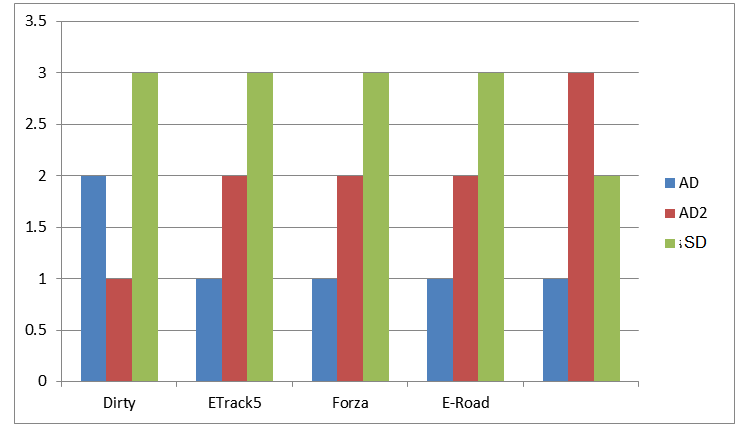
\includegraphics[width=0.9\textwidth]{fig/classement.PNG}
	\begin{minipage}{10cm}
		\centering
		\caption{\footnotesize Controllers ranking in one lap.}
		\label{clas}
	\end{minipage} 

\end{figure}
\begin{table} [h!] 
	
	\caption{Controllers results in one lap}
	\label{resulta11}
	\begin{tabular}{ |p{15.2cm}|}
		\hline
		\textbf{E-Track5}   
		\\
		\hline
	\end{tabular}
	\begin{tabular}{ |p{3cm}|p{2cm}|p{2cm}|p{2 cm}|p{2 cm}|p{2 cm}|}
		\hline
		&
		{ \color{red}\textbf{SD}}&  
		{ \color{red} \textbf{AD1} } &
		{ \color{red} \textbf{AD2} } &
		{ \color{red} \textbf{AD3} } &
		{ \color{red} \textbf{AD5} }
		\\
		\hline
		Best Time &
		01:11:58 & 01:12:69&  01:08:36 & 01:05:96 & 37:12 
		\\
		\hline
		Topspeed & 149   & 146 & 164& 168 & 199 
		\\
		\hline
		Minspeed & 59 & 59 & 67 & 61  & 116
		\\
		\hline 
		
		Damage 0 & 0 & 0 & 0 & 0 & 0 
		\\
		\hline 
		Fuel & 93:51  & 93:91 & 93:91 & 93:92 & 93:33
		\\
		\hline 
		
	\end{tabular}
	\begin{tabular}{ |p{15.2cm}|}
		\hline
		\textbf{Dir1}   
		\\
		\hline
	\end{tabular}
	\begin{tabular}{ |p{3cm}|p{2cm}|p{2cm}|p{2 cm}|p{2 cm}|p{2 cm}|}
		\hline
		&
		{ \color{red}\textbf{SD}}&  
		{ \color{red} \textbf{AD1} } &
		{ \color{red} \textbf{AD2} } &
		{ \color{red} \textbf{AD3} } &
		{ \color{red} \textbf{AD5} }
		\\
		\hline
		Lap Time &  01:20:74 & 57:87 & 01:09:19 & 58:11 & / 
		\\
		\hline
		Topspeed & 132  & 126 & 136 & 138 & /
		\\
		\hline
		Minspeed &  21 & 39 & 24 & 36 & /
		\\
		\hline 
		
		Damage &  0 & 0 & 0 & 0 & 9274 
		\\
		\hline 
		Fuel & 93:51 & 93:03 & 93:15 & 93:22 & 89:68
		\\
		\hline
		
	\end{tabular}
	
	\begin{tabular}{ |p{15.2cm}|}
		\hline
		\textbf{Froza}   
		\\
		\hline
	\end{tabular}
	\begin{tabular}{ |p{3cm}|p{2cm}|p{2cm}|p{2 cm}|p{2 cm}|p{2 cm}|}
		\hline
		&
		{ \color{red}\textbf{SD}}&  
		{ \color{red} \textbf{AD1} } &
		{ \color{red} \textbf{AD2} } &
		{ \color{red} \textbf{AD3} } &
		{ \color{red} \textbf{AD5} }
		\\
		\hline
		Lap Time &  03:10:33  & 02:48:91 & 02:46:70  & 03:17:55   & 02:08:67
		\\
		\hline
		Topspeed & 149 & 247 & 238 & 251 & 234 
		\\
		\hline
		Minspeed &  22 & 58 & 19 & -92 & 58
		\\
		\hline 
		Damage & 0 & 0 & 0 & 706 & 9
		\\
		\hline 
		Fuel & 92:17 & 77:69& 90:41& 88:60 & 60:55
		\\
		\hline 
	\end{tabular}
	\begin{tabular}{ |p{15.2cm}|}
		\hline
		\textbf{E-Road}   
		\\
		\hline
	\end{tabular}
	\begin{tabular}{ |p{3cm}|p{2cm}|p{2cm}|p{2 cm}|p{2 cm}|p{2 cm}|}
		\hline
		&
		{ \color{red}\textbf{SD}}&  
		{ \color{red} \textbf{AD1} } &
		{ \color{red} \textbf{AD2} } &
		{ \color{red} \textbf{AD3} } &
		{ \color{red} \textbf{AD5} }
		\\
		\hline
		Best Time &  02:51:25 & 02:18:31 & 02:32:39  &   02:13:23 & 01:51:81
		\\
		\hline
		Topspeed & 149  & 160 & 184 & 184  & 208
		\\
		\hline
		Minspeed & 24  & 57 &  41 & 36 &  -46
		\\
		\hline 
		
		Damage & 0 & 0 & 0 & 0 & 464 
		\\
		\hline 
		Fuel & 92:76 & 91:61  & 93:00  & 93:11& 90:55 
		\\
		\hline  
		
	\end{tabular}
	
	\begin{tabular}{ |p{15.2cm}|}
		\hline
		\textbf{CG-Speedway Number1}   
		\\
		\hline
	\end{tabular}
	
	\begin{tabular}{ |p{3cm}|p{2cm}|p{2cm}|p{2 cm}|p{2 cm}|p{2 cm}|}
		\hline
		&
		{ \color{red}\textbf{SD}}&  
		{ \color{red} \textbf{AD1} } &
		{ \color{red} \textbf{AD2} } &
		{ \color{red} \textbf{AD3} } &
		{ \color{red} \textbf{AD5} }
		\\
		\hline
		Best Time & 01:32:60   & 01:20:57 & 01:22:60 & 01:16:75 & 51:89 
		\\
		\hline
		Topspeed & 149  & 190 & 193 & 199 & 202
		\\
		\hline
		Minspeed & 38 & 58 & 38 & 55  & 53
		\\
		\hline 
		Damage & 0 & 0 & 0& 0 & 62
		\\
		\hline 
		Fuel & 93:11  & 91:72 & 93:01 & 92:61 & 92:41
		\\
		\hline 
		
	\end{tabular} 
\end{table}
\newpage

\begin{figure}[h!]
	
	\centering
	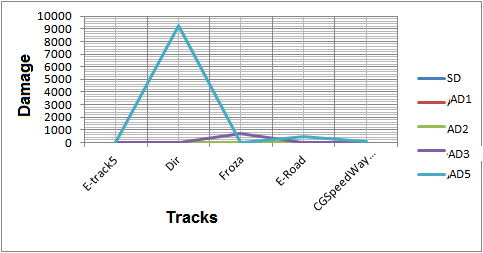
\includegraphics[width=0.9\textwidth]{fig/choc1lap.PNG}
	\begin{minipage}{10cm}
		\centering
		\caption{\footnotesize Damage rate in one lap.}
		\label{choclap}
	\end{minipage} 
\end{figure}


Figure \ref{choclap} displays the damage rate for one lap of each controller, note that the AD5 and AD3 controllers  have the highest damage values especially in Dirty tracks and Type "oval" but in the tracks ("CGSpeedWayNumber1", "Roed-E", "Froza") we do not have too much risk.

\newpage


\subsubsection{ Five lap race:}	
In this phase, we will do the same but with 5 laps for each track (see table \ref {Tabtrack}) and got the following results (see table \ref{resulta12} ). \\

\begin{table} [h!] 
	
	\caption{Results of five laps race}
	\label{resulta12}
	\begin{tabular}{ |p{15.2cm}|}
		\hline
		\textbf{E-Track5}   
		\\
		\hline
	\end{tabular}
	\begin{tabular}{ |p{3cm}|p{2cm}|p{2cm}|p{2 cm}|p{2 cm}|p{2 cm}|}
		\hline
		{ \color{blue}\textbf{5 laps} }&
		{ \color{red}\textbf{SD}}&  
		{ \color{red} \textbf{AD1} } &
		{ \color{red} \textbf{AD2} } &
		{ \color{red} \textbf{AD3} } &
		{ \color{red} \textbf{AD5} }
		\\
		\hline
		Best Time & 01:05:15  & 01:21:24  &04:55:99  & 59:37 & 29:87 
		\\
		\hline
		Topspeed & 149  & 148 & 150 & 170 & 199 
		\\
		\hline
		Minspeed & 46 & 44 & 60 & 78 & 172 
		\\
		\hline 
		
		
		Lastlap Time  & 01:05:17 & 01:31:36 & 01:02:55 & 59:38 & 30:07
		\\
		\hline 
		Best lap & 4 & 02 & 01 & 4 & 2 
		\\
		\hline
		Damage & 0 & 0 & 0 & 0 & 0 
		\\
		\hline 
		Fuel & 71:22 & 71:25 & 77:55 & 77:26 & 77:32 
		\\
		\hline 
		Lap & 5/5 & 5/5 & 5/5 & 5/5 & 5/5
		\\
		\hline	
	\end{tabular}
	\begin{tabular}{ |p{15.2cm}|}
		\hline
		\textbf{Dir1}   
		\\
		\hline
	\end{tabular}
	
	\begin{tabular}{ |p{3cm}|p{2cm}|p{2cm}|p{2 cm}|p{2 cm}|p{2 cm}|}
		\hline
		{ \color{blue}\textbf{5 laps} }&
		{ \color{red}\textbf{SD}}&  
		{ \color{red} \textbf{AD1} } &
		{ \color{red} \textbf{AD2} } &
		{ \color{red} \textbf{AD3} } &
		{ \color{red} \textbf{AD5} }
		\\
		\hline
		Best Time & 01:12:96 & 50:48  & 02:23:12 &49:84 & 35:51 
		\\
		\hline
		Topspeed & 132  & 126 & 136 & 145 & 139 
		\\
		\hline
		Minspeed &  21 & -12 & 43 & 25 & -54 
		\\
		\hline 
		
		
		Lastlap	Time  & 01:13:08  & 55:59 & 02:23:12 & 50:64 & 01:02:91 
		\\
		\hline 
		best lap & 14 & 4 & 0 1& 2 & 5 
		\\
		\hline
		Damage &  0 & 502 & 0 & 0 & 9274 
		\\
		\hline 
		Fuel & 85:04 & 76:59 &86:69& 86:44& 86:06 
		\\
		\hline
		Lap & 5/5 & 5/5 & 1/5 & 5/5 & 5/5
		\\
		\hline		
	\end{tabular}
	\begin{tabular}{ |p{15.2cm}|}
		\hline
		\textbf{Froza}   
		\\
		\hline
	\end{tabular}
	
	
	\begin{tabular}{ |p{3cm}|p{2cm}|p{2cm}|p{2 cm}|p{2 cm}|p{2 cm}|}
		\hline
		{ \color{blue}\textbf{5 laps} }&
		{ \color{red}\textbf{SD}}&  
		{ \color{red} \textbf{AD1} } &
		{ \color{red} \textbf{AD2} } &
		{ \color{red} \textbf{AD3} } &
		{ \color{red} \textbf{AD5} }
		\\
		\hline
		Best Time & 03:02:89 & 02:39:82 & 07:14:90  & 02:47:14  & 02:20:27 
		\\
		\hline
		Topspeed & 149 & 248 & 209 & 250 & 246 
		\\
		\hline
		Minspeed & 23  & 41 & -53 & -86 & 63 
		\\
		\hline 
		
		
		Lastlap	Time  & 03:02:91 & 02:48:06 & 03:20:16 & 03:34:52 & 03:00:55
		\\
		\hline 
		Best lap & 4 & 4 & 01 & 1 & 04 
		\\
		\hline
		Damage & 0 & 0 & 2269 &2621 & 0 
		\\
		\hline 
		Fuel & 85:51 & 85:18 & 86:46 & 86:06 & 76:55
		\\
		\hline 
		Lap & 5/5 & 5/5 & 4/5 & 5/5 & 5/5
		\\
		\hline	
	\end{tabular}
\end{table}
\newpage
\begin{table}[h!]
	\begin{tabular}{ |p{15.2cm}|}
		\hline
		\textbf{E-Road}   
		\\
		\hline
	\end{tabular}
	\begin{tabular}{ |p{3cm}|p{2cm}|p{2cm}|p{2 cm}|p{2 cm}|p{2 cm}|}
		\hline
		{ \color{blue}\textbf{5 laps} }&
		{ \color{red}\textbf{SD}}&  
		{ \color{red} \textbf{AD1} } &
		{ \color{red} \textbf{AD2} } &
		{ \color{red} \textbf{AD3} } &
		{ \color{red} \textbf{AD5} }
		\\
		\hline
		Best Time & 02:44:93  & 02:11:39 & 04:55:92 & 02:09:77 & 01:25:66 
		\\
		\hline
		Topspeed & 149  & 202 & 175 & 209& 207 
		\\
		\hline
		Minspeed & 24  & -58 & -50 & -58 & -55 
		\\
		\hline 
		
		Lastlap Time  & 02:44:93 & 01:29:02 & 06:08:49 &  05:56:16  & 01:27:38 
		\\
		\hline 
		Best lap & 3 & 5 & 1& 2 & 03
		\\
		\hline
		Damage & 0 & 2013 & 3018 &  4266& 2239 
		\\
		\hline 
		Fuel & 87:97 & 92:51 & 91:00 &90:76 & 84:99 
		\\
		\hline  
		
	\end{tabular}
	
	
	\begin{tabular}{ |p{15.2cm}|}
		\hline
		\textbf{CG-Speedway Number1}   
		\\
		\hline
	\end{tabular}
	\begin{tabular}{ |p{3cm}|p{2cm}|p{2cm}|p{2 cm}|p{2 cm}|p{2 cm}|}
		\hline
		{ \color{blue}\textbf{5 laps} }&
		{ \color{red}\textbf{SD}}&  
		{ \color{red} \textbf{AD1} } &
		{ \color{red} \textbf{AD2} } &
		{ \color{red} \textbf{AD3} } &
		{ \color{red} \textbf{AD5} }
		\\
		\hline
		Best Time & 01:25:01  & 01:25:00 & 01:18:13& 01:12:24 & 53:61 
		\\
		\hline
		Topspeed & 149  & 190 & 194 & 200 & 178 
		\\
		\hline
		Minspeed & 37 & 57 & 32 & -54 & -51 
		\\
		\hline 
		
		Lastlap	Time  & 01:25:14 & 01:14:59 & 01:29:65 & 01:12:81& 01:46:47 
		\\
		\hline 
		Best lap & 3 & 3 & 2 & 2 & 02  
		\\
		\hline
		Damage & 0 & 0 & 0 & 108 & 114 
		\\
		\hline 
		Fuel & 90:51 & 91:00 & 90:76 & 84:99 & 80:65 
		\\
		\hline 
		Lap & 5/5 & 5/5& 3/5 & 5/5 & 5/5
		\\
		\hline
	\end{tabular} 
\end{table}

from Table \ref{resulta12}, we noticed that for each lap, our controller tries to minimize driving time and use a maximum speed without consuming more fuel  and decreasing damage in all tracks, it improves driving to give us more optimal results then the last lap. \\

\subsubsection{ 20 lap race:}	
In this section, we set the distance to 20 laps for each track and for each controller. \\	

\begin{table} [h!] 
	
	\caption{Results for 20 laps}
	\label{resultat1}
	\begin{tabular}{ |p{15.2cm}|}
		\hline
		\textbf{E-Track5}   
		\\
		\hline
	\end{tabular}
	\begin{tabular}{ |p{3cm}|p{2cm}|p{2cm}|p{2 cm}|p{2 cm}|p{2 cm}|}
		\hline
		{ \color{blue}\textbf{20 laps} }&
		{ \color{red}\textbf{SD}}&  
		{ \color{red} \textbf{AD1} } &
		{ \color{red} \textbf{AD2} } &
		{ \color{red} \textbf{AD3} } &
		{ \color{red} \textbf{AD5} }
		\\
		\hline
		Best Time & 01:05:15  & 01:21:24  &04:33:24  & 59:37 & 29:87 
		\\
		\hline
		Topspeed & 149  & 148 & 203 & 160 & 199 
		\\
		\hline
		Minspeed & 46 & 44 & 60 & 78 & 172 
		\\
		\hline 
		
		
		Lastlap	Time  & 01:05:17 & 01:31:36 & 01:02:55 & 59:37 & 30:07
		\\
		\hline 
		Best lap & 14 & 02 & 18 &4 & 8 
		\\
		\hline
		Damage & 0 & 0 & 0 & 0 & 0 
		\\
		\hline 
		Fuel & 71:22 & 71:25 & 77:45 & 77:45 & 77:02 
		\\
		\hline 
		Lap & 20/20 & 20/20 & 20/20 & 20/20 & 20/20
		\\
		\hline
		
	\end{tabular}
	\begin{tabular}{ |p{15.2cm}|}
		\hline
		\textbf{Dir1}   
		\\
		\hline
	\end{tabular}
	\begin{tabular}{ |p{3cm}|p{2cm}|p{2cm}|p{2 cm}|p{2 cm}|p{2 cm}|}
		\hline
		{ \color{blue}\textbf{20 laps} }&
		{ \color{red}\textbf{SD}}&  
		{ \color{red} \textbf{AD1} } &
		{ \color{red} \textbf{AD2} } &
		{ \color{red} \textbf{AD3} } &
		{ \color{red} \textbf{AD5} }
		\\
		\hline
		Best Time & 01:12:96 & 50:43  &02:23:12  & 49:84 & 35:51 
		\\
		\hline
		Topspeed & 132  & 126 & 136 & 145 & 139 
		\\
		\hline
		Minspeed &  21 & -52 & -43 & 25& -54 
		\\
		\hline 
		
		
		Lastlap	Time  & 01:13:08  & 02:33:43 & 02:23:12 & 02:23:94& 01:02:91 
		\\
		\hline 
		Best lap & 14 & 07 & 01 & 2 & 5 
		\\
		\hline
		Damage &  0 & 7438 & 1889 & 905 & 9274 
		\\
		\hline 
		Fuel & 65:04 & 79:26 & 79:98 & 79:26  & 66:06 
		\\
		\hline
		Lap & 20/20 & 14/20 & 01/20 & 11/20 & 20/20
		\\
		\hline
	\end{tabular}
	
	\begin{tabular}{ |p{15.2cm}|}
		\hline
		\textbf{Froza}   
		\\
		\hline
	\end{tabular}
	\begin{tabular}{ |p{3cm}|p{2cm}|p{2cm}|p{2 cm}|p{2 cm}|p{2 cm}|}
		\hline
		{ \color{blue}\textbf{20 laps} }&
		{ \color{red}\textbf{SD}}&  
		{ \color{red} \textbf{AD1} } &
		{ \color{red} \textbf{AD2} } &
		{ \color{red} \textbf{AD3} } &
		{ \color{red} \textbf{AD5} }
		\\
		\hline
		Best Time & 03:03:66  & 02:39:82 & 07:14:90  & 02:47:14  & 02:20:27 
		\\
		\hline
		Topspeed & 149 & 248 & 209 & 250 & 246 
		\\
		\hline
		Minspeed & 22  & -41 & -53 & -86 & 63 
		\\
		\hline 
		
		
		Lastlap	Time  & 03:03:66 & 02:47:26 & 09:55:62 & 03:14:23 & 09:21:23
		\\
		\hline 
		Best lap & 20 & 04 & 01 & 2 & 04 
		\\
		\hline
		Damage & 0 & 468 & 2269 & 9704 & 0 
		\\
		\hline 
		Fuel & 62:61 & 71:88 & 60:55 & 65:85 & 60:55
		\\
		\hline 
		Lap & 20/20 & 20/20 & 04/20 & 20/20 & 20/20
		\\
		\hline
	\end{tabular}
\end{table}
\newpage
\begin{table} [h!]
	
	\begin{tabular}{ |p{15.2cm}|}
		\hline
		\textbf{E-Road}   
		\\
		\hline
	\end{tabular}
	
	\begin{tabular}{ |p{3cm}|p{2cm}|p{2cm}|p{2 cm}|p{2 cm}|p{2 cm}|}
		\hline
		{ \color{blue}\textbf{20 laps} }&
		{ \color{red}\textbf{SD}}&  
		{ \color{red} \textbf{AD1} } &
		{ \color{red} \textbf{AD2} } &
		{ \color{red} \textbf{AD3} } &
		{ \color{red} \textbf{AD5} }
		\\
		\hline
		Best Time & 02:44:93  & 02:11:39 & 04:33:59 & 01:85:16 & 01:25:66 
		\\
		\hline
		Topspeed & 149  & 202 & 203 & 150 & 207 
		\\
		\hline
		Minspeed & 24  & -58 & 32& -58 & -55 
		\\
		\hline 
		
		Lastlap	Time  & 02:45:08 & 03:00:20 & 04:51:53 & 05:34:85  & 01:27:38 
		\\
		\hline 
		Best lap & 3 & 3 & 17 & 2& 03
		\\
		\hline
		Damage & 0 & 6056 & 7309 &9602  & 2239 
		\\
		\hline 
		Fuel & 62:11 & 78:25 & 79:25 &  72:01 & 55:22 
		\\
		\hline  
		Lap & 20/20 & 9/20 &20/20 & 10/20 & 20/20
		\\
		\hline
	\end{tabular}
	\begin{tabular}{ |p{15.2cm}|}
		\hline
		\textbf{CG-Speedway Number1}   
		\\
		\hline
	\end{tabular}
	\begin{tabular}{ |p{3cm}|p{2cm}|p{2cm}|p{2 cm}|p{2 cm}|p{2 cm}|}
		
		{ \color{blue}\textbf{20 laps} }&
		{ \color{red}\textbf{SD}}&  
		{ \color{red} \textbf{AD1} } &
		{ \color{red} \textbf{AD2} } &
		{ \color{red} \textbf{AD3} } &
		{ \color{red} \textbf{AD5} }
		\\
		\hline
		Best Time & 01:25:00  & 01:12:99 & 01:12:23& 01:12:24 & 53:61 
		\\
		\hline
		Topspeed & 149  & 191& 194 & 200 & 178 
		\\
		\hline
		Minspeed & 49 & 57 & 32 & -53 & -51 
		\\
		\hline 
		
		Lastlap	Time  & 01:25:01 & 01:12:99& 01:29:65 & 03:15:39 & 01:46:47 
		\\
		\hline 
		Best lap & 12 & 20 & 02 &07  & 02  
		\\
		\hline
		Damage & 0 & 0 & 0 & 1790 & 114 
		\\
		\hline 
		Fuel & 66:66 & 62:58 & 73:38 &75:66 & 60:65 
		\\
		\hline 
		Lap & 20/20 & 20/20 & 03/20 & 13/20 & 20/20
		\\
		\hline
	\end{tabular} 
	\label{Result1r}
\end{table}

The table (\ref{Result1r} ) above shows that among the five drivers, the minimum time has been reached by the AD5 controller in each of the five tracks, this was due to the steering unit of the target. The target position allows the car to adjust safely the required steering angle  with the maximum speed so the controller AD5 gave the best time.
\\
However, taking a smaller target angle required a greater distance to cover by car by taking a less efficient trajectory. In addition, the number of times the car was off the road on Dir1 and Forza was higher for AD5 and, accordingly, the time that the car has passed out of the track was potentially higher than the other controllers.
\\	

Thus, higher damages happened after the collision with the outer walls of the track when the car is off the track. The simple driver SD driver and AD1, AD2 AD3 especially got less damage compared the version of AD5. The simple SD driver finished the race without damage, while AD5 was able to complete all the tracks safely except the Dir1t4 and Forza circuit where the damage is a little high for the AD3 driver (fig.\ref{resultat1}) .But the result may be more favourable than the other results by SD, DA1, DA2.\\
For the fuel consumption depends percentage of shocks and category of circuits.

\subsubsection{Time trial races for 2 seconds}

Now, we set the race stopping criterion to 2s and TORCS takes a decision in 0.02s (20 ms) so each controller is tested 100 actions.
we got the results that are shown in Figure \ref{steertst}  and Figure \ref{steertst2}  which represent the change in the target angle and "steer" function for each controller in a second.



We have noticed:\\\\
-The Trajectory of the target angle in SD controllers, AD1, AD2, AD3 are almost identical and the same for 2 seconds in a road type of track (see fig. \ref{angleresultat} ).\\
-According to Figure \ref{steertst},  the car seems to be lost in the first seconds while  the steer of the AD5 controller has a constant value. \\

\begin{figure}[h!]
	
	\centering
	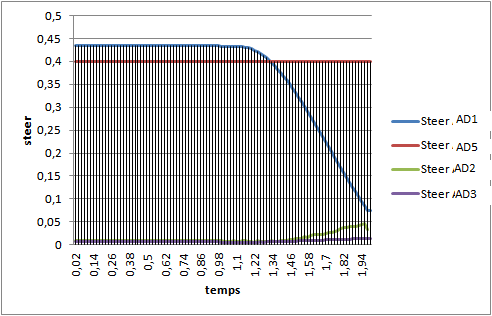
\includegraphics[width=0.9\textwidth]{fig/steertest.PNG}
	\begin{minipage}{10cm}
		\centering
		\caption{\footnotesize  Steer values for 2seconds in CG speedWay Number1 track}
		\label{steertst}
	\end{minipage} 
	
\end{figure}	

\begin{figure}[h!]	
	\centering
	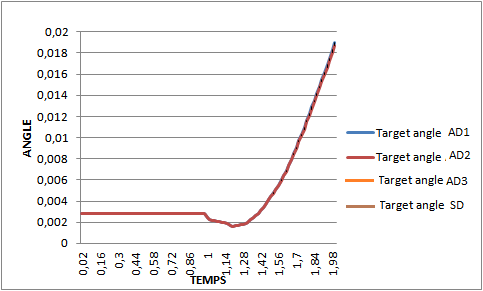
\includegraphics[width=0.9\textwidth]{fig/angletest.PNG}
	\begin{minipage}{10cm}
		\centering
		\caption{\footnotesize   Target angle variations for 2 s in CG speedWay Number1 rack }
		\label{steertst2}
	\end{minipage} 
	\index{tracé}                     %% inclure le mot tracé dans l'index
	\index{fonction}                  %% include le mot fonction dans l'index
	
\end{figure}
\subsubsection{Time trial races for 1 minute}

Now, we set the race stopping criterion to 60s and TORCS. The results are in table\ref{resulta2} and Figures Fig.\ref{steer5min} , Fig.\ref{accel/brake}, Fig.\ref{gear1min}.

\begin{table} [h!] 
	
	\caption{Results of the controllers in 1 minute time trial race}
	\label{resulta2}
	\begin{tabular}{ |p{13,8cm}|}
		\hline
		\textbf{E-Track5}   
		\\
		\hline
	\end{tabular}
	\begin{tabular}{ ||p{3cm}||p{3cm}||p{3cm}||p{3 cm}||}
		\hline
		{ \color{blue}\textbf{} }&
		{ \color{red}\textbf{Best Time} }&
		{ \color{red} \textbf{Distance } } &
		{ \color{red} \textbf{Top speed} }
		\\
		\hline
		AD1 &00:00  &810,865& 152 
		\\
		\hline
		AD2 & 00:00 &1304,172& 149
		\\
		\hline
		AD3 &00:00 & 5202,99& 154 
		\\
		\hline 
		AD5 & 29:20 &	489  & 198
		\\
		\hline 
		
	\end{tabular}
	\begin{tabular}{ |p{13,8cm}|}
		\hline
		\textbf{Dir1}   
		\\
		\hline
	\end{tabular}
	\begin{tabular}{ ||p{3cm}||p{3cm}||p{3cm}||p{3 cm}||}
		\hline
		{ \color{blue}\textbf{} }&
		{ \color{red}\textbf{Best Time} }&
		{ \color{red} \textbf{Distance } } &
		{ \color{red} \textbf{Top speed} }
		\\
		\hline
		AD1 & 57:52 & 3260,43&  166
		\\
		\hline
		AD2 & 00:00 & 1156,22
		& 137
		\\
		\hline
		AD3 & 00:00 & 2934& 139
		\\
		\hline 
		AD5 & 00:00 &	827 & 153
		\\
		\hline 
		
	\end{tabular}
	\begin{tabular}{ |p{13,8cm}|}
		\hline
		\textbf{Froza}   
		\\
		\hline
	\end{tabular}
	\begin{tabular}{ ||p{3cm}||p{3cm}||p{3cm}||p{3 cm}||}
		\hline
		{ \color{blue}\textbf{} }&
		{ \color{red}\textbf{Best Time} }&
		{ \color{red} \textbf{Distance(m) } } &
		{ \color{red} \textbf{Top speed(m/s)} }
		\\
		\hline
		AD1 & 02:49:12  &17352,3  &  247
		\\
		\hline
		AD2 & 02:49:12  & 17354,12 & 239
		\\
		\hline
		AD3 & 03:44:56 & 17355 & 205 
		\\
		\hline 
		AD5 & 57:66 & 17355,2 & 203 
		\\
		\hline 
		
	\end{tabular}
	\begin{tabular}{ |p{13,8cm}|}
		\hline
		\textbf{E-Road}   
		\\
		\hline
	\end{tabular}
	\begin{tabular}{ ||p{3cm}||p{3cm}||p{3cm}||p{3 cm}||}
		\hline
		{ \color{blue}\textbf{} }&
		{ \color{red}\textbf{Best Time} }&
		{ \color{red} \textbf{Distance } } &
		{ \color{red} \textbf{Top speed} }
		\\
		\hline
		AD1 & 00:00 &1630 &  160
		\\
		\hline
		AD2 & 00:00 & 1304 & 170 
		\\
		\hline
		AD3 & 00:00  &2282& 174
		\\
		\hline 
		AD5 & 01:00:00 & 3260 & 199
		\\
		\hline 
		
	\end{tabular}
	\begin{tabular}{ |p{13,8cm}|}
		\hline
		\textbf{CG-Speedway Number1}   
		\\
		\hline
	\end{tabular}
	\begin{tabular}{ ||p{3cm}||p{3cm}||p{3cm}||p{3 cm}||}
		\hline
		{ \color{blue}\textbf{} }&
		{ \color{red}\textbf{Best Time} }&
		{ \color{red} \textbf{Distance } } &
		{ \color{red} \textbf{Top speed} }
		\\
		\hline
		AD1 & 00:00 & 1654&  175
		\\
		\hline
		AD2 & 00:00  & 620,25& 160 
		\\
		\hline
		AD3 & 00:00  &1860,75&184 
		\\
		\hline 
		AD5 & 54:22& 2687,75 &200
		\\
		\hline 
		
	\end{tabular}
\end{table}
\newpage
\begin{figure}[h!]
	
	\centering
	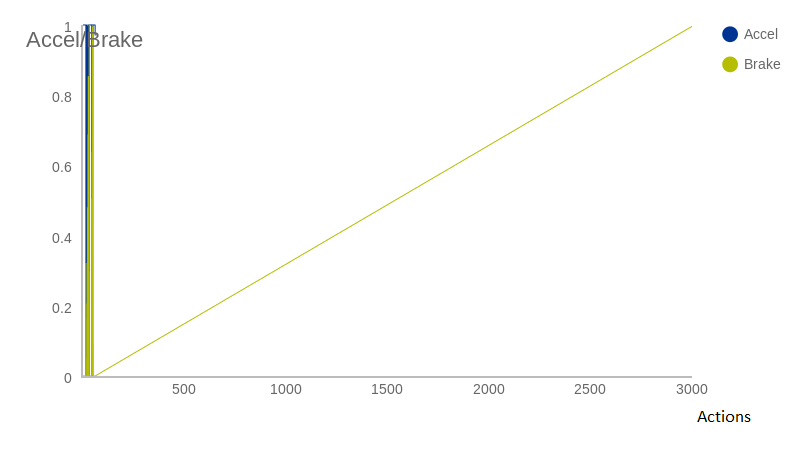
\includegraphics[width=0.4\textwidth]{fig/AD5Accel.PNG}
	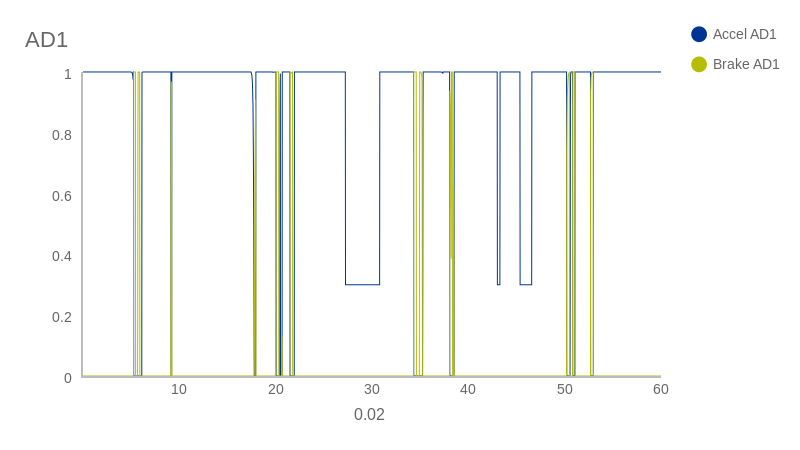
\includegraphics[width=0.4\textwidth]{fig/AD1accel.PNG}
	\begin{minipage}{10cm}
		\centering
		\caption{\footnotesize Acceleration and brake values of AD5 and D1 in 1 minute race(CG-SpeedWay Number1 track)..}
		\label{accel/brake}
	\end{minipage} 
	
\end{figure}
\begin{figure}[h!]
	
	\centering
	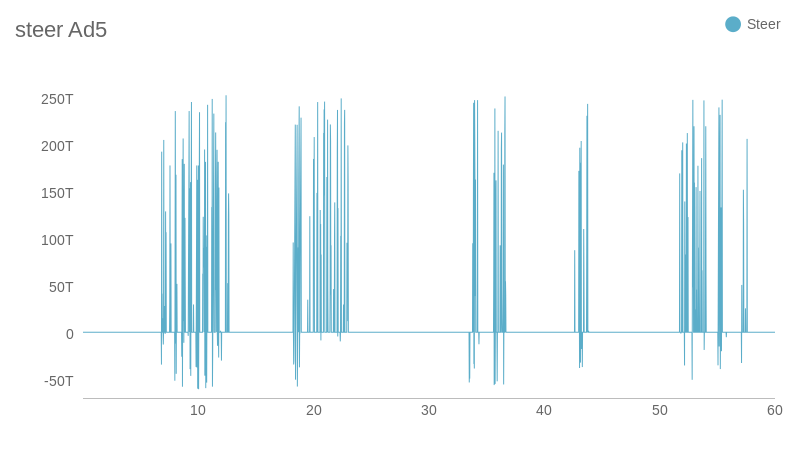
\includegraphics[width=0.4\textwidth]{fig/AD5steer.PNG}
	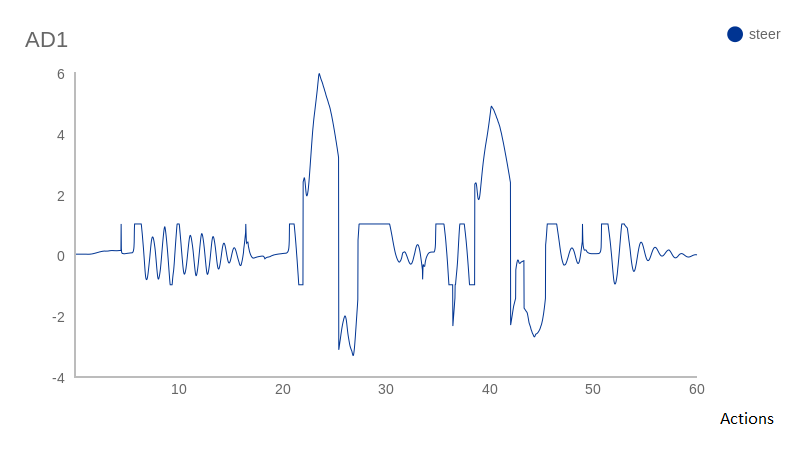
\includegraphics[width=0.4\textwidth]{fig/AD1steer.PNG}
	\begin{minipage}{10cm}
		\centering
		\caption{\footnotesize Steer values for of AD5 and D1 in 1 minute race(CG-SpeedWay Number1 track).}
		\label{steer5min}
	\end{minipage} 
	\index{tracé}                     %% inclure le mot tracé dans l'index
	\index{fonction}                  %% include le mot fonction dans l'index
	
\end{figure}

\begin{figure}[h!]
	
	\centering
	\includegraphics[width=0.8\textwidth]{fig/AD1gear.PNG}
	
	\begin{minipage}{10cm}
		\centering
		\caption{\footnotesize Gear values for of AD5 and D1 in 1 minute race(CG-SpeedWay Number1 track). }
		\label{gear1min}
	\end{minipage} 
                 %% include le mot fonction dans l'index
	
\end{figure}

According to the figures above (Fig.\ref{steer5min} , Fig. \ref{accel/brake}, Fig. \ref{gear1min} ) and Table \ref{resulta2} , we deduce that the AD5 controller remains the most stable than other .only in special cases the other controllers can have better results.

\newpage
\subsubsection{Time trial races for 5 minutes}
Now, we set the race stopping criterion to 300s and TORCS. The results are in Table\ref{resulta9})


\begin{table} [h!] 
	
	\caption{Results of the controllers in 5 minute time trial race}
	\label{resulta9}
	\begin{tabular}{ |p{13,8cm}|}
		\hline
		\textbf{E-Track5}   
		\\
		\hline
	\end{tabular}
	\begin{tabular}{ ||p{3cm}||p{3cm}||p{3cm}||p{3 cm}||}
		\hline
		{ \color{blue}\textbf{} }&
		{ \color{red}\textbf{Best Time} }&
		{ \color{red} \textbf{Distance } } &
		{ \color{red} \textbf{Top speed} }
		\\
		\hline
		AD1 &01:11:98  &4540,844&  155
		\\
		\hline
		AD2 & 02:15:26 &8803,161& 155
		\\
		\hline
		AD3 & 02:13:46 &20233,85 & 160 
		\\
		\hline 
		AD5 & 29:30&32600&199 
		\\
		\hline 
		
	\end{tabular}
	\begin{tabular}{ |p{13,8cm}|}
		\hline
		\textbf{Dir1}   
		\\
		\hline
	\end{tabular}
	\begin{tabular}{ ||p{3cm}||p{3cm}||p{3cm}||p{3 cm}||}
		\hline
		{ \color{blue}\textbf{} }&
		{ \color{red}\textbf{Best Time} }&
		{ \color{red} \textbf{Distance } } &
		{ \color{red} \textbf{Top speed} }
		\\
		\hline
		AD1 & 52:27 & 7825,032&126  
		\\
		\hline
		AD2 & 00:00 &5202,99& 134
		\\
		\hline
		AD3 & 00:00 & 652& 145
		\\
		\hline 
		AD5 & 00:00 &620,25& 153 
		\\
		\hline 
		
	\end{tabular}
	\begin{tabular}{ |p{13,8cm}|}
		\hline
		\textbf{Froza}   
		\\
		\hline
	\end{tabular}
	\begin{tabular}{ ||p{3cm}||p{3cm}||p{3cm}||p{3 cm}||}
		\hline
		{ \color{blue}\textbf{} }&
		{ \color{red}\textbf{Best Time} }&
		{ \color{red} \textbf{Distance(m) } } &
		{ \color{red} \textbf{Top speed(m/s)} }
		\\
		\hline
		AD1 & 02:49:12  &17352,3  &  247
		\\
		\hline
		AD2 & 02:49:12  & 17354,12 & 239
		\\
		\hline
		AD3 & 03:44:56 & 17355 & 205 
		\\
		\hline 
		AD5 & 57:66 & 17355,2 & 203 
		\\
		\hline 
		
	\end{tabular}
	\begin{tabular}{ |p{13,8cm}|}
		\hline
		\textbf{E-Road}   
		\\
		\hline
	\end{tabular}
	\begin{tabular}{ ||p{3cm}||p{3cm}||p{3cm}||p{3 cm}||}
		\hline
		{ \color{blue}\textbf{} }&
		{ \color{red}\textbf{Best Time} }&
		{ \color{red} \textbf{Distance } } &
		{ \color{red} \textbf{Top speed} }
		\\
		\hline
		AD1 & 03:62:33 & 11586,2 &  160
		\\
		\hline
		AD2 & 02:41:41  & 11588 & 208 
		\\
		\hline
		AD3 & 02:13:73 & 23136,4& 210
		\\
		\hline 
		AD5 & 01:15:16 & 23139 & 217
		\\
		\hline 
		
	\end{tabular}
	\begin{tabular}{ |p{13,8cm}|}
		\hline
		\textbf{CG-Speedway Number1}   
		\\
		\hline
	\end{tabular}
	\begin{tabular}{ ||p{3cm}||p{3cm}||p{3cm}||p{3 cm}||}
		\hline
		{ \color{blue}\textbf{} }&
		{ \color{red}\textbf{Best Time} }&
		{ \color{red} \textbf{Distance } } &
		{ \color{red} \textbf{Top speed} }
		\\
		\hline
		AD1 & 01:15:19 & 23136 &  195
		\\
		\hline
		AD2 & 01:15:80 & 17352,2 & 193 
		\\
		\hline
		AD3 & 01:10:20 & 28920,4 &200 
		\\
		\hline 
		AD5 & 44:67& 28921,6 &206 
		\\
		\hline 
		
	\end{tabular}
\end{table}
\newpage



\subsection{Real race}
\subsubsection{5 laps race}
In this case, we test our controller "AD5", without considering the variables and opponents sensors.\\

Our main goal is to test the performance of "AD5" in a race, and answer the following questions: Could we have a perfect driving in a race with "AD5" only with the track borders sensors? Can we win the race with AD5?\\
In this context we tested "AD5" in 5 tracks see Table \ref{Tabtrack} and for the opponents, we chose from the following cars (see table \ref {resultat30} ).
\\

\begin{table}[h!]
	
	\caption{TORCS teams and cars}
	\label{resultat30}
	\begin{tabular}{ |p{1cm}|p{2cm}|p{5cm}|p{6 cm}|}
		\hline
		{ \color{red}\textbf{Num} }&
		{ \color{red}\textbf{Team}}&  
		{ \color{red} \textbf{Drivers } } &
		{ \color{red} \textbf{Cars} }
		\\
		\hline
		1  & \textbf{berwin} & berwin 1,
		berwin 2,
		berwin 3,
		berwin 4,
		berwin 5,
		berwin 6,
		berwin 7,
		berwin 8,
		berwin 9,
		berwin 10
		& 
		car1-stock1,
		car1-stock1, car1-trb1,
		car2-trb1,
		car3-trb1,
		car4-trb1,
		car5-trb1,
		car6-trb1,
		car7-trb1,
		car1-trb3,
		\\
		\hline
		2 & \textbf{bt} & bt1
		bt2
		,bt3
		,bt4
		,bt5
		,bt6
		,bt7
		,bt8
		,bt9
		,bt10.
		
		&
		car1-stock1,
		car1-stock1, car1-trb1,
		car2-trb1,
		car3-trb1,
		car4-trb1,
		car5-trb1,
		car6-trb1,
		car7-trb1,
		car1-trb3, 
		\\
		\hline
		3 & \textbf{damned} & damned1
		,damned2
		,damned3
		,damned4
		,damned5
		,damned6
		,damned7
		,damned8
		,damned9
		,damned10
		.
		& 
		Ford Fucus WRC-offroad-4WD GrA,
		Peugeot 206 WRC -offroad-4WD GrA,
		Peugeot 306 Maxi -offroad-4WD GrA,
		Mitsibishi lancer -offroad-4WD GrA,
		Subaru Inperza -offroad-4WD GrA,,
		Toyata Corolla -offroad-4WD GrA,
		car5-trb1,
		car6-trb1,
		car7-trb1,
		car1-trb3.  
		\\
		\hline 
		4 & \textbf{inferno} & inferno1,
		inferno2,
		inferno3,
		inferno4,
		inferno5,
		inferno6,
		inferno7,
		inferno8,
		inferno9,
		inferno10.
		&
		Car1-ows1,
		Peugeot 406-Track FWD Grb,
		car1-trb1,
		car2-trb1,
		car3-trb1,
		car4-trb1,
		car5-trb1,
		car6-trb1,
		car7-trb1,
		car1-trb3.
		\\
		\hline 
		5 & \textbf{tita} & tita1,
		tita2,
		tita3,
		tita4,
		tita5,
		tita6,
		tita7,
		tita8,
		tita9,
		tita10.
		& 
		Car1-ows1,
		Peugeot 406-Track FWD Grb,
		car1-trb1,
		car2-trb1,
		car3-trb1,
		car4-trb1,
		car5-trb1,
		car6-trb1,
		car7-trb1,
		car1-trb3. 
		\\
		\hline 
		
	\end{tabular} 
	
\end{table}
\newpage

After the launch of the race "AD5" against the 10 cars of each team (list in table \ref{resultat30}) for 5 laps in each track we obtained the following results (see table \ref{resultat31})
\begin{table}[h!]
	\caption{Results of AD5  in a real race}
	\label{resultat31}
	\begin{tabular}{ |p{3cm}|p{2cm}|p{2cm}|p{2 cm}|p{2 cm}|p{2 cm}|}
		\hline
		{ \color{blue}\textbf{E-Track5} }&
		{ \color{red}\textbf{Against berwin team }}&  
		{ \color{red} \textbf{Against bt team} } &
		{ \color{red} \textbf{Against damned team} } &
		{ \color{red} \textbf{Against inferno team} }&
		{ \color{red} \textbf{Against tita team} }
		\\
		\hline
		Ranking & 1/11 & 2/11   & 1/11 & 7/11& 4/11
		\\
		\hline
		race time & 02:36:78 & 02:40:38+ 03:41   & 02:42:73 & 02:15:81 + lap & 02:18:74 + 28:19
		\\
		\hline
		Best time & 29:90 & 30:28   & 30:28 & 30:59& 30:53 
		\\
		\hline 
		Maxspeed & 198 & 198 &  198 & 199 & 198
		\\
		\hline
		
		Damage & 2267 & 7939 &  5888 & 5232& 8043
		\\
		\hline 
		
		
		Pit stops & 0& 0  & 0 & 0 & 0
		\\
		\hline 	
		Lap & 5/5 & 5/5  & 5/5 & 4/5 & 5/5
		\\
		\hline
	\end{tabular} 
	\begin{tabular}{ |p{3cm}|p{2cm}|p{2cm}|p{2 cm}|p{2 cm}|p{2 cm}|}
		\hline
		{ \color{blue}\textbf{CG-SpeedWay Number1} }&
		{ \color{red}\textbf{Against berwin team }}&  
		{ \color{red} \textbf{Against bt team} } &
		{ \color{red} \textbf{Against damned team} } &
		{ \color{red} \textbf{Against inferno team} }&
		{ \color{red} \textbf{Against tita team} }
		\\
		\hline
		Ranking  & 11/11  & 11/11  & 11/11  & 11/11& 11/11
		\\
		\hline
		Race time & 03:39:12 + 44:76 & 03:34:00 + 43:19 & 03:34:75 + Lap & 02:59:83 + 3 Lap   & 03:01:75 + 4 laps
		\\
		\hline
		Best time& 46:16   & 48:56 & 47:23 & 46:06 & 03:41:41
		\\
		\hline 
		Maxspeed & 205 & 202 & 199 & 200 & 198
		\\
		\hline
		Damage &  5533 & 3096 & 3093 & 5501& 0
		\\
		\hline 
		
		
		Pit stops & 0 & 0 & 0 & 0& 0
		\\
		\hline 	
		Lap & 5/5  & 5/5 & 4/5 & 2/5 & 1/5
		\\ 
		\hline
	\end{tabular} 
	
	\begin{tabular}{ |p{3cm}|p{2cm}|p{2cm}|p{2 cm}|p{2 cm}|p{ 2 cm}|}
		\hline
		{ \color{blue}\textbf{E-Road} }&
		{ \color{red}\textbf{Against berwin team }}&  
		{ \color{red} \textbf{Against bt team} } &
		{ \color{red} \textbf{Against damned team} } &
		{ \color{red} \textbf{Against inferno team} }&
		{ \color{red} \textbf{Against tita team} }
		\\
		\hline
		Ranking  & 11/11 & 11/11 & 11/11 & 11/11 & 11/11
		\\
		\hline
		Race time & 06:00:00 +lap & 06:14:64 +3lap & 06:13:26 +2 Laps  &  04:50:42 +2lap  & 04:56:16 +3lap
		\\
		\hline
		Race time & 01:21:29  & 02:19:92 & 01:39:54 & 01:27:27   & 01:48:18
		\\
		\hline 
		Maxspeed & 205 & 201 & 212 & 211 & 208
		\\
		\hline
		
		Damage & 9979 & 10362 & 4421 & 7685 & 5593
		\\
		\hline 
		
		
		Pit stops & 0 & 0 & 0 & 0 & 0
		\\
		\hline 	
		Lap & 4/5 & 2/5 & 3/5 & 3/5 &  2/5
		\\
		\hline
	\end{tabular} 
\end{table} 
\newpage
\begin{table}[h!]
	\begin{tabular}{ |p{3cm}|p{2cm}|p{2cm}|p{2 cm}|p{2 cm}|p{2 cm}|}
		\hline
		{ \color{blue}\textbf{Froza} }&
		{ \color{red}\textbf{Against berwin team }}&  
		{ \color{red} \textbf{Against bt team} } &
		{ \color{red} \textbf{Against damned team} } &
		{ \color{red} \textbf{Against inferno team} }&
		{ \color{red} \textbf{Against tita team} }
		\\
		\hline
		Ranking & 10/11  & 11/11 & 11/11 & 10/11& 10/11
		\\
		\hline
		Race time & 7:44:99 + Lap & 8:07:39 + 02:16:32 & 08:09:42 + 1Lap & 6:40:33 + Lap 0 &  6:37:02 + Lap 
		\\
		\hline
		Best time & 01:57:58 & 01:45:30 & 02:03:00 & 02:04:00& 02:04:37
		\\
		\hline 
		Maxspeed & 243  & 282 & 260 & 220& 217
		\\
		\hline
		
		Damage & 2275 & 95 & 475 & 416 & 1185
		\\
		\hline 
		
		
		Pit stops & 0 & 0 & 0 & 0 & 0
		\\
		\hline 
		Lap & 4/5 & 5/5  & 4/5 & 4/5& 4/5 
		\\
		\hline	
	\end{tabular} 
	
	
	\begin{tabular}{ |p{3cm}|p{2cm}|p{2cm}|p{2 cm}|p{2 cm}|p{2 cm}|}
		\hline
		{ \color{blue}\textbf{Dir1} }&
		{ \color{red}\textbf{Against berwin team }}&  
		{ \color{red} \textbf{Against bt team} } &
		{ \color{red} \textbf{Against damned team} } &
		{ \color{red} \textbf{Against inferno team} }&
		{ \color{red} \textbf{Against tita team} }
		\\
		\hline
		Ranking  & 11/11 & 11/11 & 11/11 & 11/11& 10/11
		\\
		\hline
		Race time & 03:03:41+ 5 laps & 02:55:54 + 5 laps & 03:05:90 + 5 laps & 02:55:54 + 5 laps & 02:48:12+ 4 Laps
		\\
		\hline
		Best time & 00:00  & 00:00 & 00:00 & 00:00 & 00:00
		\\
		\hline 
		Maxspeed & 146 & 141 & 145 & 145 & 145
		\\
		\hline
		
		Damage & 10017 & 6462 & 39 & 226& 271
		\\
		\hline 
		
		
		Pit stops & 0 & 0 & 0 & 0 & 0					\\
		\hline 	
	\end{tabular} 
	
\end{table}
\paragraph{\\}	
From Table \ref {resultat31}, we noticed that our controller has won a race only in some types of tracks such as "E-track5" category "Oval track" and only against some car types like cars of category "stock1" ,"ows","trb".
\\

In some cases on other roads, our controller gives us the best results, but in a very short time, for example in the beginning of the race in the E-Road track, against the berwin team or our bt controller could go first turn by a ranking between "1 and 4" and a maximum speed equal to 199 but it has little damage when the other cars overtaken it.
\\

When our controller is in parallel with his opponent, and the distance between them is smaller, and they are in a smaller width track,  there is a possibility of  damage (see fig.\ref{damages} ).
\\

According to Fig. \ref{damages1}  despite our controller can win the race on the E-track5 but it had a higher crash rates in the majority of cases.

\newpage
\begin{figure}[h!]
	
	\centering
	\includegraphics[width=1\textwidth]{fig/damageRace.PNG}
	\begin{minipage}{10cm}
		\centering
		\caption{\footnotesize Damage values of AD5 in E-track5.}
		\label{damages}
	\end{minipage} 
\end{figure}

Figure \ref{speed} shows the different values of the speed of our AD controller 5 against some TORCS teams in E-track5, we observed that in the majority of cases our car is very slow compared to the other cars in each team. \\

\begin{figure}[h!]
	
	\centering
	\includegraphics[width=1.1\textwidth]{fig/SpeedRace.PNG}
	\begin{minipage}{10cm}
		\centering
		\caption{\footnotesize Speed Variation of AD 5 in E-track5.}
		\label{speed}
	\end{minipage} 
	
	
\end{figure}
\subsection{Real race with ow1 car}
To validate our controllers results, we replace our race car by another car  "OW1". We have run each of our controllers against a car from each team after tests yielded the following results: \\	

\subsubsection{AD1 in one lap race}
Table \ref{resultat33}  displays the AD1 Controller test results in a race, it was noted that he can not win the race and there are some difficulties for example it can not  overtake a car without damage in a curve, and sometimes it can not finish the race until the end.

\begin{table}[h!]
	\caption{AD1 in one lap race with ow1  car}
	\label{resultat33}
	\begin{tabular}{ |p{3cm}|p{2cm}|p{2cm}|p{2 cm}|p{2 cm}|p{2 cm}|}
		\hline
		{ \color{blue}\textbf{Froza} }&
		{ \color{red} \textbf{ AD 1} } &
		{ \color{red}\textbf{ berwin1 }}&  
		{ \color{red} \textbf{bt 2 } } &
		
		{ \color{red} \textbf{inferno 3} }
		&{ \color{red} \textbf{tita 4} }
		\\
		\hline
		Ranking  & 5/5  & 2/5 & 01/5 & 03/5& 4/5
		\\
		\hline
		Race time & 01:45:26 + 58:49 & 01:45:26 + 02:10 & 01:45:26  & 1:45:26 + 02:35 &  1:45:26 + 02:50 
		\\
		\hline
		Best time & 02:43:58 & 01:47:37 & 01:45:26 & 01:47:62& 01:47:76
		\\
		\hline 
		Maxspeed & 299  & 287 & 280 & 289 & 289
		\\
		\hline
		
		Damage & 321 & 0 & 489 & 390 & 0
		\\
		\hline 
		
		
		Pit stops & 0 & 0 & 0 & 0 & 0
		\\
		\hline 
		Lap & 1/1 & 1/1  & 1/1 & 1/1& 1/1 
		\\
		\hline	
	\end{tabular} 
	
	
	
\end{table}


\subsubsection{AD2 in one lap race}	
The following table \ref{resultat32} shows that in one lap, although the AD2 controller does not give the best results but at least guarantee correct behaviour with minimum shock rate and speed value maximization comparing with previous results (driving without an opponent)
\begin{table}[h!]
	\caption{Results of AD2 controller in one lap with ow1 car}
	\label{resultat32}
	\begin{tabular}{ |p{3cm}|p{2cm}|p{2cm}|p{2 cm}|p{2 cm}|p{2 cm}|}
		\hline
		{ \color{blue}\textbf{Froza} }&
		{ \color{red} \textbf{ AD 2} } &
		{ \color{red}\textbf{ berwin1 }}&  
		{ \color{red} \textbf{bt 2 } } &
		
		{ \color{red} \textbf{inferno 3} }
		&{ \color{red} \textbf{tita 4} }
		\\
		\hline
		Ranking  & 5/5  & 1/5 & 02/5 & 03/5& 4/5
		\\
		\hline
		Race time &  01:40:59+ 01:03:71 & 01:40:59  &  01:40:59 + 04:08  &  01:40:59 + 04:34 &   01:40:59 + 04:74 
		\\
		\hline
		Best time & 02:44:31 &  01:40:59 & 01:44:68 & 01:44:93& 01:45:34
		\\
		\hline 
		Maxspeed & 244  & 297 & 284 & 284 & 282
		\\
		\hline
		
		Damage & 0 & 0 & 18 & 796 & 1198
		\\
		\hline 
		
		
		Pit stops & 0 & 0 & 0 & 0 & 0
		\\
		\hline 
		Lap & 1/1 & 1/1  & 1/1 & 1/1& 1/1 
		\\
		\hline	
	\end{tabular} 
	
	
	
\end{table}
\newpage

\subsubsection{AD3 in one lap race}	
as Table \ref {resultat35} shows, we have the same comments mentioned above with a risk of not finishing the race since the damage is very high in a short distance.

\begin{table}[h!]
	\caption{Results of AD3 controller in one lap with ow1 car}
	\label{resultat35}
	\begin{tabular}{ |p{3cm}|p{2cm}|p{2cm}|p{2 cm}|p{2 cm}|p{2 cm}|}
		\hline
		{ \color{blue}\textbf{Froza} }&
		{ \color{red} \textbf{ AD 3} } &
		{ \color{red}\textbf{ berwin1 }}&  
		{ \color{red} \textbf{bt 2 } } &
		
		{ \color{red} \textbf{inferno 3} }
		&{ \color{red} \textbf{tita 4} }
		\\
		\hline
		Ranking  & 5/5  & 4/5 & 01/5 & 02/5& 3/5
		\\
		\hline
		Race time &  01:44:81+ 01:02:99 & 01:44:81+ 03:62  &  01:44:81   &  01:40:59 + 01:02 &   01:40:59 + 02:78 
		\\
		\hline
		Best lap & 02:47:80 &  01:48:44 & 01:44:81 & 01:45:83& 01:47:6
		\\
		\hline 
		Maxspeed & 315  & 287 & 282 & 293 & 280
		\\
		\hline
		
		Damage & 319 & 196 & 9 & 709 & 1192
		\\
		\hline 
		
		
		Pit stops & 0 & 0 & 0 & 0 & 0
		\\
		\hline 
		Lap & 1/1 & 1/1  & 1/1 & 1/1& 1/1 
		\\
		\hline	
	\end{tabular} 
	
\end{table}
\subsubsection{AD5 in one lap race}
In this case, we noticed the same problems except that an improvement in time and speed (see table. \ref{resultat34} )
\begin{table}[h!]
	\caption{Results of AD5 controller in one lap with ow1 car}
	\label{resultat34}
	\begin{tabular}{ |p{3cm}|p{2cm}|p{2cm}|p{2 cm}|p{2 cm}|p{2 cm}|}
		\hline
		{ \color{blue}\textbf{Froza} }&
		{ \color{red} \textbf{ AD 5} } &
		{ \color{red}\textbf{ berwin1 }}&  
		{ \color{red} \textbf{bt 2 } } &
		
		{ \color{red} \textbf{inferno 3} }
		&{ \color{red} \textbf{tita 4} }
		\\
		\hline
		Ranking  & 5/5  & 1/5 & 02/5 & 03/5& 4/5
		\\
		\hline
		Race time &  01:39:28 +26:23 &  01:39:28  &  01:39:28 + 4:69   &  01:39:28 + 04:87 &   01:39:28 + 10:45 
		\\
		\hline
		Best time & 02:05:51 & 01:39:28 & 01:43:97 & 01:44:83& 01:49:47
		\\
		\hline 
		Maxspeed & 255  & 306 & 297 & 286 & 273
		\\
		\hline
		
		Damage & 289 & 0 & 427 & 563 & 277
		\\
		\hline 
		
		
		Pit stops & 0 & 0 & 0 & 0 & 0
		\\
		\hline 
		Lap & 1/1 & 1/1  & 1/1 & 1/1& 1/1 
		\\
		\hline	
	\end{tabular} 
	
\end{table}

\subsubsection{AD5 with opponents sensors}

After adding the opponents sensors in the AD5  controller, we obtained the following results after 20 laps on the E-Track5 track :

\begin{table} [h!] 
	
	\caption{Results of AD5 with and without opponents sensors in E-Track5}
	\label{resulta101}
	\begin{tabular}{ |p{12cm}|}
		\hline
		{ \color{red}	\textbf{AD5 without opponents sensors} }
		\\
		\hline
	\end{tabular}
	
	\begin{tabular}{|p{4cm}||p{1cm}||p{1cm}||p{1cm}||p{1cm}||p{1cm}||p{1cm}||p{1cm}|}
		\hline
		\textbf{Laps}&1 & 2& 3& 4&5&... & 20 
		\\
		\hline
		\textbf{Distance}&1621,73&3243,46&4865,19&6486,92&8108,65
		& ...&32434,6 
		\\
		\hline
		\textbf{Damage}&0 &0& 0& 0&0&... &0
		\\
		\hline
		\textbf{Time}&0 &0& 0& 0&0&... &0
		\\
		\hline
		\textbf{Speed}&0 &0& 0& 0&0&... &0
		\\
		\hline
	\end{tabular}
	\begin{tabular}{ |p{12cm}|}
		\hline
		{ \color{red}	\textbf{with opponents sensors}   }
		\\
		\hline
		
	\end{tabular}
	
	\begin{tabular}{|p{4cm}||p{1cm}||p{1cm}||p{1cm}||p{1cm}||p{1cm}||p{1cm}||p{1cm}|}
		\hline
		\textbf{Laps}&1 & 2& 3& 4&5&... & 20 
		\\
		\hline
		\textbf{Distance}&1621,73&3243,46&4865,19&6486,92&8108,65
		& ...&32434,6  
		\\
		\hline
		\textbf{Damage}&0 &0& 0& 0&0&... &0
		\\
		\hline
		\textbf{Time}&0 &0& 0& 0&0&... &0
		\\
		\hline
		\textbf{Speed}&0 &0& 0& 0&0&... &0
		\\
		\hline
	\end{tabular}
\end{table}
\newpage
%	\section{Conclusion}
%
%		At the end of this chapter, we got an automatic controller architecture and controller of intelligent behavior which automatic driving in "TORCS". The design of intelligent controller that is using fuzzy logic in several approaches.
%		Thus the design stage is complete, the system is ready to perform and then to test it.\\	
%		
%After a series of tests, we got the final version of our controller with an optimal setting for a simple and healthy behavior
\bibliography{biblio}





\end{document}
